\section{Solution techniques for the Poisson equation}
\label{SEC_SCARC_solver}

Commonly used approaches for the solution of the Poisson equation (\ref{EQ_SCARC_pressure}) 
 are either based on direct or iterative solution strategies which will be described in more detail subsequently. Their efficient parallelization must bridge the gap between the following two very conflicting requirements:
\begin{itemize}
\item {\bf Efficient convergence behavior} ('Globality' preferred)\\
Especially for globally coupled systems such as elliptic equations fast convergence is essentially based on how well an algorithm is able to reproduce global dependencies. Powerful elliptic solvers mainly rest on highly recursive algorithmic structures which strongly couple the overall data of the whole domain. Thus, they have very little inherent parallelism. 
\item {\bf Good parallelization properties} ('Locality' preferred)\\
In contrast to that, methods with a high degree of parallelism often possess a strongly local character. In the ideal case they only need local communication between neighboring subdomains which can nowadays be performed with high computational efficiency on modern parallel platforms.  
\end{itemize}
%This can be summarized in the following statement:
%`Well parallelizable algorithms for elliptic problems are often numerically inefficient, numerically efficient algorithms are hardly parallelizable.'


For single-mesh applications the strongly recursive design of traditional elliptic solvers very well reflects the fast and globally acting character of the pressure. In this case, all data required during the computations are easily accessible in the storage of the only processor in use which allows a high computational efficiency. 

For multi-mesh applications the first obvious idea consists in the development of a 1-to-1 parallel analog by splitting up the serial structures according to the new decomposition. But in this case, all required recursive data would be distributed across the entire computing system and would have to be exchanged very frequently which is extremely inefficient from a computational point of view.
In order to increase the degree of parallelism the only remedy is to modify existing techniques or to develop completely new strategies, which are better adapted to modern parallel architectures. However, this process is necessarily associated with a loosening of the global coupling.
New local information can no longer be distributed globally just when it is needed, but only with a time delay or, in order to save computational overhead, only in  reduced or coarser form. Typically, this leads to dependencies on the number of subdomains or the grid resolution associated with losses of numerical efficiency and possible troubles in the correct mapping of actual physical processes. 




% ------------------------------------------------------------------------------------------------------------------------------------------
% Direct solvers
% ------------------------------------------------------------------------------------------------------------------------------------------
\subsection{Direct solvers} 
\label{SEC_SCARC_direct_solvers}
At a first glance, the ongoing improvements in the current computer technology motivate the use of direct methods such as the Gaussian elimination method and its variants for symmetric, positive definite matrices for the solution of the elliptic equations. Another extremely powerful class of direct methods which is successfully used in many different branches of science is based on spectral solvers. 
Both classes will be explained in more detail below.

Direct solvers compute the solution of a system of equations within a possibly very complex step without intermediate approximations. They may be performed with enormous speed and are often used for the demonstration of potential computer power, see e.g.\ the LINPACK-tests by~\cite{Dongarra:1998}.
They have proven to be very robust even in the non-symmetric and ill-conditioned case. Besides, they are nearly independent of the  degree of grid distortion (except for rounding errors) and well suited for the application on unstructured grids.  
In contrast to iterative methods, they are completely independent of whether a good starting solution exists or not, but they also do not benefit if this is already the case. They achieve a high level of computational accuracy, but they do not benefit if this is not required at all.

However, as already mentioned, the development of corresponding parallel analogues is highly complicated.
Most often, reasonably efficient strategies follow purely algebraic considerations
and are not conforming with geometrically motivated domain decompositions strategies.
Nevertheless, for  moderately sized problems, especially if only one or a few sub-meshes are used, direct solvers are incomparably fast and should generally be preferred over iterative ones.
Typically, there is a critical number of subdomains for which the parallelization overhead dominates the numerical efficiency associated with the original serial methodology which should be analyzed carefully.
 
 

% ------------------------------------------------------------------------------------------------------------------------------------------
% FFT solver
% ------------------------------------------------------------------------------------------------------------------------------------------
\subsubsection{Current FFT pressure solver}
\label{SEC_SCARC_fft_solver}

Spectral solvers like the {\it Fast Fourier Transformation} (FFT) exploit a very special property of the underlying Poisson problem, namely that sine and cosine functions are eigenvectors of the Laplace operator. They expand the solution as a Fourier series which can be quickly performed at rather low complexity. In practice, this approach has proven to be highly efficient and is used in many different fields of application. However, FFT methods are restricted to structured grids which may impede the use for complex geometries.

As described in detail in the FDS Technical Guide~\cite{McGrattan:2018:TG}, the pressure equation (\ref{EQ_SCARC_pressure}) is obtained from the momentum equation by a sequence of substitutions and simplifications. The major advantage of this derivation is that it finally leads to a system of equations which has constant coefficients (i.e.\ is separable). 
Since FDS furthermore relies on the use of cubic meshes each with structured rectangular grids each, it is possible to use a highly optimized FFT solver from the CRAYFISHPAK~\cite{Sweet::Crayfishpak}.
%
In the single-mesh case only one globally acting FFT-method is performed which has proven to be extremely powerful and fast over the past years. 
In the multi-mesh case every sub-mesh performs its own local FFT in order to compute an exact solution to the related local Poisson problem as illustrated in Fig.~\ref{FIG_SCARC_local_ffts}. The global solution is then composed from the local ones.
\begin{figure}[ht]
\begin{center}
\begin{tikzpicture}
[
scale=0.6,
every node/.style={scale=0.6},
Background/.style={rectangle,draw=black!04,fill=black!04, thin, minimum size = 4 cm},
Obstruction/.style={rectangle,draw=black!70,fill=black!40, very thick, minimum size=1cm},
Finegrid/.style={step=0.5cm,gray,very thin},
Thickline/.style={-,draw=black!100,fill=black!02, very thick},
Thinline/.style={draw=black!100,fill=black!02, very thin},
Ball/.style={circle, draw=black!40, fill=red!20, thin, minimum size=3.5mm},
Circle/.style={circle,draw=black!40,fill=black!06,thin,minimum size=35.5mm},
Rectangle/.style={rectangle,draw=black!10,fill=white,inner xsep=0pt, inner ysep=0pt,},
Box/.style= {very thin, rectangle, inner xsep=10pt, inner ysep=10pt,},
ComArrow/.style= {<->,very thick, draw=red!70,},
DotArrow/.style= {<-, thick, dotted, draw=black!70,},
]

\node[Background] at (  2,2) {};
\node[Background] at (  6,2) {};
\node[Background] at (  6,6) {};
\node[Background] at (10,6) {};

\node[Obstruction] at (2,2) {};

\draw[Finegrid] (0,0) grid (  8,4);
\draw[Finegrid] (4,4) grid (12,8);

\draw[Thickline] (0,0)--(  8,0);
\draw[Thickline] (4,8)--(12,8);
\draw[Thickline] (0,4)--(  4,4);
\draw[Thickline] (8,4)--(12,4);

\draw[Thickline] (  0,0)--(  0,4);
\draw[Thickline] (  4,8)--(12,8);
\draw[Thickline] (  4,4)--(  4,8);
\draw[Thickline] (  8,0)--(  8,4);
\draw[Thickline] (12,4)--(12,8);

\draw[Thickline] (4,0)--(4,4);
\draw[Thickline] (4,4)--(8,4);
\draw[Thickline] (8,4)--(8,8);

\node[Rectangle] at (  2,2.0) {\Large \begin{tabular}{c} Local \\ FFT\end{tabular}};
\node[Rectangle] at (  6,2.0) {\Large \begin{tabular}{c} Local \\ FFT\end{tabular}};
\node[Rectangle] at (  6,6.0) {\Large \begin{tabular}{c} Local \\ FFT\end{tabular}};
\node[Rectangle] at (10,6.0) {\Large \begin{tabular}{c} Local \\ FFT\end{tabular}};

\draw[ComArrow](3.2,2)--(4.8,2);
\draw[ComArrow](6,3.2)--(6,4.8);
\draw[ComArrow](7.2,6)--(8.8,6);

\draw [DotArrow] (8.1,5.6) -- (10.0,2.4);
\draw [DotArrow] (7.0,3.8) -- (  9.5,1.6);
\draw [DotArrow] (4.1,0.7) -- (  9.5,0.7);

\node [Box] (box) at (11.2,1.5){%
    \begin{minipage}{0.36\textwidth}
    \begin{center}
        {\Large Artificial \\[1ex]
           boundaries}
    \end{center}
    \end{minipage}};

\draw[ComArrow](-5.2,6)--(-3.6,6);
\node [Box,red!70] (box) at (-0.4,6){%
    \begin{minipage}{0.56\textwidth}
    \begin{center}
        {\Large Local communication}
    \end{center}
    \end{minipage}};

\end{tikzpicture}

\caption[Mesh-wise FFT-methods]{Mesh-wise FFT-methods for the 2D pipe geometry: First each mesh performs its own local FFT method to compute the solution of the respective local Poisson problem. Then, the global solution results from the composition of the local solutions.}
\label{FIG_SCARC_local_ffts}
\end{center}
\end{figure}

A drawback associated with this approach is that the mathematical solvability of the local problems requires the definition of appropriate boundary conditions all over the local boundary, i.e.\ along the new artificial boundaries between the single meshes where the true boundary conditions are not known at all. Instead, they are only approximately defined as Dirichlet boundary values, consisting of the mean values of neighboring cells in adjacent meshes taken from the last time step, which may lead to losses of accuracy.
%
On the other hand, this strictly local oriented approach possesses an extremely high parallel efficiency because the exchange of the internal boundary values only requires next-neighbor communications which can be performed with great computational efficiency on today's parallel architectures.

As already described, the most fundamental characteristic of the pressure equation (\ref{EQ_SCARC_pressure})  is a very fast propagation speed for information. Only a single time step may suffice to spread new pressure information over the whole computational domain, i.e.\ local effects or perturbations have immediate impact on the overall solution. 

Due to the purely local character of the mesh-wise FFT-solver, however, new information can only be transferred mesh-by-mesh, successively using the data exchanges between adjacent meshes  as illustrated in Fig.~\ref{FIG_SCARC_mesh_wise_transfer}.
%
This necessarily involves a time delay compared to the real physical propagation speed and brings dependencies on the number of subdomains into play.
The higher the number of subdomains and the associated artificial fragmentation of the global connectivity is, the stronger this effect may be with corresponding negative impacts on the accuracy and stability of the whole method.
Nevertheless, for small numbers of subdomains this effect has proven to be very weak and the efficiency of the local FFT-methodology mainly dominates.

\begin{center}
\begin{figure}[ht]
\begin{minipage}{4.3cm}
\begin{tikzpicture}
[
scale=0.32,
every node/.style ={scale=0.32},
Background/.style={rectangle,draw=black!04,fill=black!04, thin, minimum size = 4 cm},
BackgroundInflow/.style={rectangle,draw=black!04,fill={rgb,255:red,73;green,137;blue,162},opacity=0.3, thin, minimum size = 4 cm},
Obstruction/.style={rectangle,draw=black!70,fill=black!40, very thick, minimum size=1cm},
Finegrid/.style={step=0.5cm,gray,very thin},
Thickline/.style={-,draw=black!100,fill=black!02, very thick},
Thinline/.style={draw=black!100,fill=black!02, very thin},
Inflow/.style={-,draw={rgb,255:red,73;green,137;blue,162},line width=0.8mm},
Inarrow/.style={->,draw={rgb,255:red,73;green,137;blue,162},thin},
Outflow/.style={-,draw=blue!60,,line width=0.8mm},
Ball/.style={circle, draw=black!40, fill=red!20, thin, minimum size=3.5mm},
Circle/.style={circle,draw=black!40,fill=black!06,thin,minimum size=35.5mm},
Rectangle/.style={rectangle,draw=black!10,fill=white,inner xsep=0pt, inner ysep=0pt,},
Box/.style= {very thin, rectangle, inner xsep=10pt, inner ysep=10pt,},
ComArrow/.style={<->,semithick,draw=red!70},
]

\node[BackgroundInflow] at (2,2) {};
\node[Background] at (6,2) {};
\node[Background] at (6,6) {};
\node[Background] at (10,6) {};

\node[Obstruction] at (2,2) {};

\draw[Finegrid] (0,0) grid (8,4);
\draw[Finegrid] (4,4) grid (12,8);

\draw[Thickline] (0,0)--(8,0);
\draw[Thickline] (4,8)--(12,8);
\draw[Thickline] (0,4)--(4,4);
\draw[Thickline] (8,4)--(12,4);

\draw[Thickline] (0,0)--(0,4);
\draw[Thickline] (4,8)--(12,8);
\draw[Thickline] (4,4)--(4,8);
\draw[Thickline] (8,0)--(8,4);
\draw[Thickline] (12,4)--(12,8);

\draw[Thickline] (4,0)--(4,4);
\draw[Thickline] (4,4)--(8,4);
\draw[Thickline] (8,4)--(8,8);

\draw[Inflow]   (0,1.5)--(0,2.5);
\draw[Inarrow]  (-1.5,1.6)--(-0.25,1.6);
\draw[Inarrow]  (-1.5,2.0)--(-0.25,2.0);
\draw[Inarrow]  (-1.5,2.4)--(-0.25,2.4);
%\draw[Outflow]  (12,4)--(12,8);

%\draw[ComArrow](3.0,2)--(5.0,2);

\node [Box] (Box) at (6.0,9.0){{\HUGE 1. cycle}};

\end{tikzpicture}

\end{minipage}
\begin{minipage}{3.9cm}
\begin{tikzpicture}
[
scale=0.32,
every node/.style ={scale=0.32},
Background/.style={rectangle,draw=black!04,fill=black!04, thin, minimum size = 4 cm},
BackgroundInflow/.style={rectangle,draw=black!04,fill={rgb,255:red,73;green,137;blue,162},opacity=0.3, thin, minimum size = 4 cm},
Obstruction/.style={rectangle,draw=black!70,fill=black!40, very thick, minimum size=1cm},
Finegrid/.style={step=0.5cm,gray,very thin},
Thickline/.style={-,draw=black!100,fill=black!02, very thick},
Thinline/.style={draw=black!100,fill=black!02, very thin},
Inflow/.style={-,draw={rgb,255:red,73;green,137;blue,162},line width=0.8mm},
Inarrow/.style={->,draw={rgb,255:red,73;green,137;blue,162},thin},
Outflow/.style={-,draw=blue!60,,line width=0.8mm},
Ball/.style={circle, draw=black!40, fill=red!20, thin, minimum size=3.5mm},
Circle/.style={circle,draw=black!40,fill=black!06,thin,minimum size=35.5mm},
Rectangle/.style={rectangle,draw=black!10,fill=white,inner xsep=0pt, inner ysep=0pt,},
Box/.style= {very thin, rectangle, inner xsep=10pt, inner ysep=10pt,},
ComArrow/.style={<->,semithick,draw=red!70},
]

\node[BackgroundInflow] at (2,2) {};
\node[BackgroundInflow] at (6,2) {};
\node[Background] at (6,6) {};
\node[Background] at (10,6) {};

\node[Obstruction] at (2,2) {};

\draw[Finegrid] (0,0) grid (8,4);
\draw[Finegrid] (4,4) grid (12,8);

\draw[Thickline] (0,0)--(8,0);
\draw[Thickline] (4,8)--(12,8);
\draw[Thickline] (0,4)--(4,4);
\draw[Thickline] (8,4)--(12,4);

\draw[Thickline] (0,0)--(0,4);
\draw[Thickline] (4,8)--(12,8);
\draw[Thickline] (4,4)--(4,8);
\draw[Thickline] (8,0)--(8,4);
\draw[Thickline] (12,4)--(12,8);

\draw[Thickline] (4,0)--(4,4);
\draw[Thickline] (4,4)--(8,4);
\draw[Thickline] (8,4)--(8,8);

\draw[Inflow]   (0,1.5)--(0,2.5);
%\draw[Inarrow]  (-1,1.6)--(-0.25,1.6);
%\draw[Inarrow]  (-1,2.0)--(-0.25,2.0);
%\draw[Inarrow]  (-1,2.4)--(-0.25,2.4);
%\draw[Outflow]  (12,4)--(12,8);

\draw[ComArrow](3.0,2)--(5.0,2);

\node [Box] (Box) at (6.0,9.0){{\HUGE 2. cycle}};

\end{tikzpicture}

\end{minipage}
\begin{minipage}{3.9cm}
\begin{tikzpicture}
[
scale=0.32,
every node/.style ={scale=0.32},
Background/.style={rectangle,draw=black!04,fill=black!04, thin, minimum size = 4 cm},
BackgroundInflow/.style={rectangle,draw=black!04,fill={rgb,255:red,73;green,137;blue,162},opacity=0.3, thin, minimum size = 4 cm},
Obstruction/.style={rectangle,draw=black!70,fill=black!40, very thick, minimum size=1cm},
Finegrid/.style={step=0.5cm,gray,very thin},
Thickline/.style={-,draw=black!100,fill=black!02, very thick},
Thinline/.style={draw=black!100,fill=black!02, very thin},
Inflow/.style={-,draw={rgb,255:red,73;green,137;blue,162},line width=0.8mm},
Inarrow/.style={->,draw={rgb,255:red,73;green,137;blue,162},thin},
Outflow/.style={-,draw=blue!60,,line width=0.8mm},
Ball/.style={circle, draw=black!40, fill=red!20, thin, minimum size=3.5mm},
Circle/.style={circle,draw=black!40,fill=black!06,thin,minimum size=35.5mm},
Rectangle/.style={rectangle,draw=black!10,fill=white,inner xsep=0pt, inner ysep=0pt,},
Box/.style = {very thin, rectangle, inner xsep=10pt, inner ysep=10pt,},
ComArrow/.style= {<->,semithick,draw=red!70},
]

\node[BackgroundInflow] at (2,2) {};
\node[BackgroundInflow] at (6,2) {};
\node[BackgroundInflow] at (6,6) {};
\node[Background] at (10,6) {};

\node[Obstruction] at (2,2) {};

\draw[Finegrid] (0,0) grid (8,4);
\draw[Finegrid] (4,4) grid (12,8);

\draw[Thickline] (0,0)--(8,0);
\draw[Thickline] (4,8)--(12,8);
\draw[Thickline] (0,4)--(4,4);
\draw[Thickline] (8,4)--(12,4);

\draw[Thickline] (0,0)--(0,4);
\draw[Thickline] (4,8)--(12,8);
\draw[Thickline] (4,4)--(4,8);
\draw[Thickline] (8,0)--(8,4);
\draw[Thickline] (12,4)--(12,8);

\draw[Thickline] (4,0)--(4,4);
\draw[Thickline] (4,4)--(8,4);
\draw[Thickline] (8,4)--(8,8);

\draw[Inflow]   (0,1.5)--(0,2.5);
%\draw[Inarrow]  (-1,1.6)--(-0.25,1.6);
%\draw[Inarrow]  (-1,2.0)--(-0.25,2.0);
%\draw[Inarrow]  (-1,2.4)--(-0.25,2.4);
%\draw[Outflow]  (12,4)--(12,8);

\draw[ComArrow](3.0,2)--(5.0,2);
\draw[ComArrow](6,3.0)--(6,5.0);

\node [Box] (Box) at (6.0,9.0){{\HUGE 3. cycle}};


\end{tikzpicture}

\end{minipage}
\begin{minipage}{3.9cm}
\begin{tikzpicture}
[
scale=0.32,
every node/.style ={scale=0.32},
Background/.style={rectangle,draw=black!04,fill=black!04, thin, minimum size = 4 cm},
BackgroundInflow/.style={rectangle,draw=black!04,fill={rgb,255:red,73;green,137;blue,162},opacity=0.3, thin, minimum size = 4 cm},
Obstruction/.style={rectangle,draw=black!70,fill=black!40, very thick, minimum size=1cm},
Finegrid/.style={step=0.5cm,gray,very thin},
Thickline/.style={-,draw=black!100,fill=black!02, very thick},
Thinline/.style={draw=black!100,fill=black!02, very thin},
Inflow/.style={-,draw={rgb,255:red,73;green,137;blue,162},line width=0.8mm},
Inarrow/.style={->,draw={rgb,255:red,73;green,137;blue,162},thin},
Outflow/.style={-,draw=blue!60,,line width=0.8mm},
Ball/.style={circle, draw=black!40, fill=red!20, thin, minimum size=3.5mm},
Circle/.style={circle,draw=black!40,fill=black!06,thin,minimum size=35.5mm},
Rectangle/.style={rectangle,draw=black!10,fill=white,inner xsep=0pt, inner ysep=0pt,},
Box/.style= {very thin, rectangle, inner xsep=10pt, inner ysep=10pt,},
ComArrow/.style= {<->,semithick,draw=red!70},
]

\node[BackgroundInflow] at (2,2) {};
\node[BackgroundInflow] at (6,2) {};
\node[BackgroundInflow] at (6,6) {};
\node[BackgroundInflow] at (10,6) {};

\node[Obstruction] at (2,2) {};

\draw[Finegrid] (0,0) grid (8,4);
\draw[Finegrid] (4,4) grid (12,8);

\draw[Thickline] (0,0)--(8,0);
\draw[Thickline] (4,8)--(12,8);
\draw[Thickline] (0,4)--(4,4);
\draw[Thickline] (8,4)--(12,4);

\draw[Thickline] (0,0)--(0,4);
\draw[Thickline] (4,8)--(12,8);
\draw[Thickline] (4,4)--(4,8);
\draw[Thickline] (8,0)--(8,4);
\draw[Thickline] (12,4)--(12,8);

\draw[Thickline] (4,0)--(4,4);
\draw[Thickline] (4,4)--(8,4);
\draw[Thickline] (8,4)--(8,8);

\draw[Inflow]   (0,1.5)--(0,2.5);
%\draw[Inarrow]  (-1,1.6)--(-0.25,1.6);
%\draw[Inarrow]  (-1,2.0)--(-0.25,2.0);
%\draw[Inarrow]  (-1,2.4)--(-0.25,2.4);
%\draw[Outflow]  (12,4)--(12,8);

\draw[ComArrow](3.0,2)--(5.0,2);
\draw[ComArrow](6,3.0)--(6,5.0);
\draw[ComArrow](7.0,6)--(9.0,6);

\node [Box] (Box) at (6.0,9.0){{\HUGE 4. cycle}};

\end{tikzpicture}

\end{minipage}
\caption[Delayed information transfer of the mesh-wise FFT solver]{Delayed information transfer of the mesh-wise FFT solver for the 2D pipe geometry: New information can only be passed across the whole domain by successively using the next-neighbor communications between adjacent meshes.}
\label{FIG_SCARC_mesh_wise_transfer}
\end{figure}
\end{center}



There is yet another important issue regarding the treatment of internal obstructions that should be considered:
Since the use of the FFT-solver is basically limited to structured meshes, it is not possible to specify internal boundary conditions and the velocity field may penetrate into internal solids as already explained in Section (\ref{SEC_SCARC_poisson}). 
%
In order to compensate this undesired effect an additional iterative correction strategy based on a {\it Direct Forcing Immersed Boundary Method}~\cite{Fadlun:2000} is used in FDS: In every time step the mesh-wise FFT algorithm is not applied only once but multiple times until a specified {\it velocity tolerance} for the remaining velocity error along internal obstructions has been reached. This iterative corrective process will be denoted as {\it pressure iteration} below.

Furthermore, although the pressure term $\cH$ is continuous at mesh interfaces, the finite-difference of its gradient is not such that the normal components of velocity also may be different at common mesh interfaces. Thus, the above pressure iteration is also used to drive the velocity normals to match up to the specified velocity tolerance along common mesh interfaces.

For both, the internal obstructions and the mesh interfaces, the required velocity tolerance and the maximum allowed number of correction iterations can be specified by the quantities {\ct VELOCITY\_TOLERANCE} and {\ct  MAX\_PRESSURE\_ITERATIONS} 
in the {\ct \&PRES}-namelist. By default, a velocity tolerance of ''characteristic mesh size'' divided by 10 and a maximum of 10 iterations is used. Fig.~\ref{FIG_SCARC_multi_pipe_fft_presite} illustrates this procedure graphically.
More detailed information about the underlying procedure can be obtained in the FDS Technical Reference Guide~\cite{McGrattan:2018:TG}.

\begin{figure}[ht]
\begin{center}
\begin{tikzpicture}
[
scale=0.6,
every node/.style={scale=0.6},
Background/.style={rectangle,draw=black!04,fill=black!04, thin, minimum size = 4 cm},
Obstruction/.style={rectangle,draw=black!70,fill=black!40, very thick, minimum size=1cm},
Finegrid/.style={step=0.5cm,gray,very thin},
Thickline/.style={-,draw=black!100,fill=black!02, very thick},
Thinline/.style={draw=black!100,fill=black!02, very thin},
Ball/.style={circle, draw=black!40, fill=red!20, thin, minimum size=3.5mm},
Circle/.style={circle,draw=black!40,fill=black!06,thin,minimum size=35.5mm},
Rectangle/.style={rectangle,draw=black!10,fill=white,inner xsep=0pt, inner ysep=0pt,},
Box/.style= {very thin, rectangle, inner xsep=10pt, inner ysep=10pt,},
DotBox/.style= {very thick, rectangle, inner xsep=0pt, inner ysep=8pt, dotted, fill=white, draw=black!70,},
ComArrow/.style= {<->,very thick, draw=red!70,},
DotArrow/.style= {<-, thick, dotted, draw=black!70,},
DotLine/.style= {very thick, dotted, draw=black!70,},
]

\node[Background] at (  2,2) {};
\node[Background] at (  6,2) {};
\node[Background] at (  6,6) {};
\node[Background] at (10,6) {};

\node[Obstruction] at (2,2) {};

\draw[Finegrid] (0,0) grid (  8,4);
\draw[Finegrid] (4,4) grid (12,8);

\draw[Thickline] (0,0)--(  8,0);
\draw[Thickline] (4,8)--(12,8);
\draw[Thickline] (0,4)--(  4,4);
\draw[Thickline] (8,4)--(12,4);

\draw[Thickline] (  0,0)--(  0,4);
\draw[Thickline] (  4,8)--(12,8);
\draw[Thickline] (  4,4)--(  4,8);
\draw[Thickline] (  8,0)--(  8,4);
\draw[Thickline] (12,4)--(12,8);

\draw[Thickline] (4,0)--(4,4);
\draw[Thickline] (4,4)--(8,4);
\draw[Thickline] (8,4)--(8,8);

\node[Rectangle] at (  2,2.0) {\Large \begin{tabular}{c} local \\ FFT\end{tabular}};
\node[Rectangle] at (  6,2.0) {\Large \begin{tabular}{c} local \\ FFT\end{tabular}};
\node[Rectangle] at (  6,6.0) {\Large \begin{tabular}{c} local \\ FFT\end{tabular}};
\node[Rectangle] at (10,6.0) {\Large \begin{tabular}{c} local \\ FFT\end{tabular}};

\draw[ComArrow](3.2,2)--(4.8,2);
\draw[ComArrow](6,3.2)--(6,4.8);
\draw[ComArrow](7.2,6)--(8.8,6);

\draw[ComArrow](-5.2,6)--(-3.6,6);
\node [Box,red!70] (box) at (-0.4,6){%
    \begin{minipage}{0.56\textwidth}
    \begin{center}
        {\Large Local communication}
    \end{center}
    \end{minipage}};

\draw[  -,DotLine](6,-0.5)--(6,-1.5);
\draw[  -,DotLine](6,-1.5)--(16,-1.5);
\draw[  -,DotLine](16,-1.5)--(16,9.5);
\draw[  -,DotLine](6,9.5)--(16,9.5);
\draw[->,DotLine](6,9.5)--(6,8.2);

\node [DotBox] (box) at (15.8,1.3){%
    \begin{minipage}{0.73\textwidth}    
    \begin{center}
    \begin{tabular}{lclc|c|}
       {\ct  \Large $err_{interfaces}$} & {\Large <} & {\ct \large VELOCITY\_TOLERANCE?}            \\[2ex]
       {\ct  \Large $err_{obstructions}$} & {\Large <} & {\ct \large VELOCITY\_TOLERANCE?}         \\[2ex]
       {\ct  \Large $num_{iterations}$ }    &{\Large <} & {\ct \large MAX\_PRESSURE\_ITERATIONS?} \\
    \end{tabular}
    \end{center}
    \end{minipage}};

\node [Box, black!70] (box) at (11,10.2){\LARGE Pressure Iteration};

\end{tikzpicture}

\caption[Mesh-wise FFT-methods with pressure correction]{Repeated use of the FFT pressure solver for a 2D pipe geometry: In the scope of a surrounding pressure iteration the mesh-wise FFT's are performed multiple times until the error related to the normal components of velocity along internal obstructions and mesh interfaces has been driven below a specified velocity tolerance.}
\label{FIG_SCARC_multi_pipe_fft_presite}
\end{center}
\end{figure}

Certainly, the increased number of mesh-wise FFT solutions leads to a higher computational effort. Nevertheless, for a multitude of cases, especially for relatively small mesh numbers or in steady-state like situations, only less corrective iterations are needed and convergence is achieved very quickly.
Increasing the number of subdomains may worsen the convergence and accuracy behaviour associated with a noticeable increase of computational costs.
%, possibly up to divergence at a (problem-dependent) critical number of subdomains. 

Especially, for extended geometries with a big number of meshes (i.e.\ tunnels) and/or transient boundary conditions this purely local strategy may experience difficulties to reproduce the rapid propagation of information for elliptic problems fast enough and convergence of the pressure iteration may be slow.
In particular, these situations make the development of alternative solution concepts appear necessary and have driven their development forward.

% ----------------------------------------------------------------------------------------------------------------------------------------
% LU solver
% ----------------------------------------------------------------------------------------------------------------------------------------
\subsubsection{$\boldmath{LU}$-factorization}
\label{SEC_SCARC_lu_decomposition}
Within the framework of the Gaussian elimination algorithm, many direct algorithms rely on the 'lower-upper'-factorization of the system matrix, $LU = PAQ$, 
with suitable permutation matrices $P$ and $Q$ and the triangular matrices $L$ and $U$, see Fig.~\ref{FIG_SCARC_lu_decomposition}. 
The solution of Equation (\ref{EQ_SCARC_single_system}) can then be obtained using a forward substitution step, $Ly=P^Tb$, followed by a backward substitution step, $U(Q^Tx)=y$.
If $A$ is symmetric, a {\it Cholesky factorization} $PAP^T=LL^T$ can be applied.

The whole process can be subdivided into three phases: 
(i) a {\it reordering phase}  where the matrix is analyzed to produce an ordering which allows a more efficient factorization,
(ii) a {\it factorization phase} where the $LU$-factorization is actually computed and stored, 
(iii) a {\it solution phase} where the forward and backward substitution is performed.
Typically, the factorization phase (ii) requires the most computing time while the solution phase (iii) is an order of magnitude faster.

\begin{figure}[ht]
\begin{center}
\begin{tikzpicture}
[ 
  every node/.style ={scale=0.35},
 ]
\tikzstyle{every path}=[draw, line width=0.3mm];
\def\bracket{
  \draw[-] (1,10) -| (0,0) -- (1,0);
  \draw[-] (9,10) -| (10,0) -- (9,0);
}
\def\basecoords{ 
    \coordinate (-v1) at (1,1);
    \coordinate (-v2) at (9,1);
    \coordinate (-v3) at (9,9);
    \coordinate (-v4) at (1,9);
}
\tikzset{pics/.cd,
  my square/.style={code={\basecoords\fill [#1] (-v1) rectangle (-v3);\bracket}},
  my trileft/.style={code={\basecoords\fill [#1] (-v2) -- (-v4) -- (-v1);\bracket}},
  my triright/.style={code={\basecoords\fill [#1] (-v2) -- (-v3) -- (-v4);\bracket}}
 }

\pic[local bounding box=A,scale=0.4]  at (0,0)                              {my square={opacity=0.3,gray} };
\pic[local bounding box=B,scale=0.4,right=2 cm of A.south east] {my trileft   ={opacity=0.3,gray}};
\pic[local bounding box=C,scale=0.4,right=2 cm of B.south east] {my triright ={opacity=0.3,gray}};

\node[scale=2] (a) at ($(A.east)!0.5!(B.west)$) {$=$};
\node[scale=2] (b) at ($(B.east)!0.5!(C.west)$) {$\times$};

\node[scale=2] (At) at ([shift={(80:0.5)}]$(A.north)$) {$A$};
\node[scale=2] (Bt) at ([shift={(80:0.5)}]$(B.north)$) {$L$};
\node[scale=2] (Ct) at ([shift={(80:0.5)}]$(C.north)$) {$U$};
\end{tikzpicture}

\end{center}
\caption{Decomposition of $A$ into a lower triangular matrix $L$ and an upper triangular matrix $U$}
\label{FIG_SCARC_lu_decomposition}
\end{figure}


A main disadvantage of this approach is that less benefit can be drawn from a very convenient property of 
the Poisson matrix $A$, namely its intrinsic {\it sparsity}:
Even though $A$ has only very few non-zero entries compared to the total number of possible entries $n^2$, 
%which are grouped in single diagonal bands (7 bands in case of the 7-point stencil), 
the $LU$-factorization process leads to {\it fill-in}, i.e.\ it produces non-zero entries in $L$ and $U$ where $A$ was zero before.
This relation is illustrated in Fig.~\ref{FIG_SCARC_lu_memory_spy}.
For a simple 3D-cube geometry which is refined into $16^3$ cells it shows the sparsity pattern of the Poisson matrix $A$
and the lower triangular matrix $L$ of its $LU$-decomposition.

\begin{figure}[ht]
\begin{center}
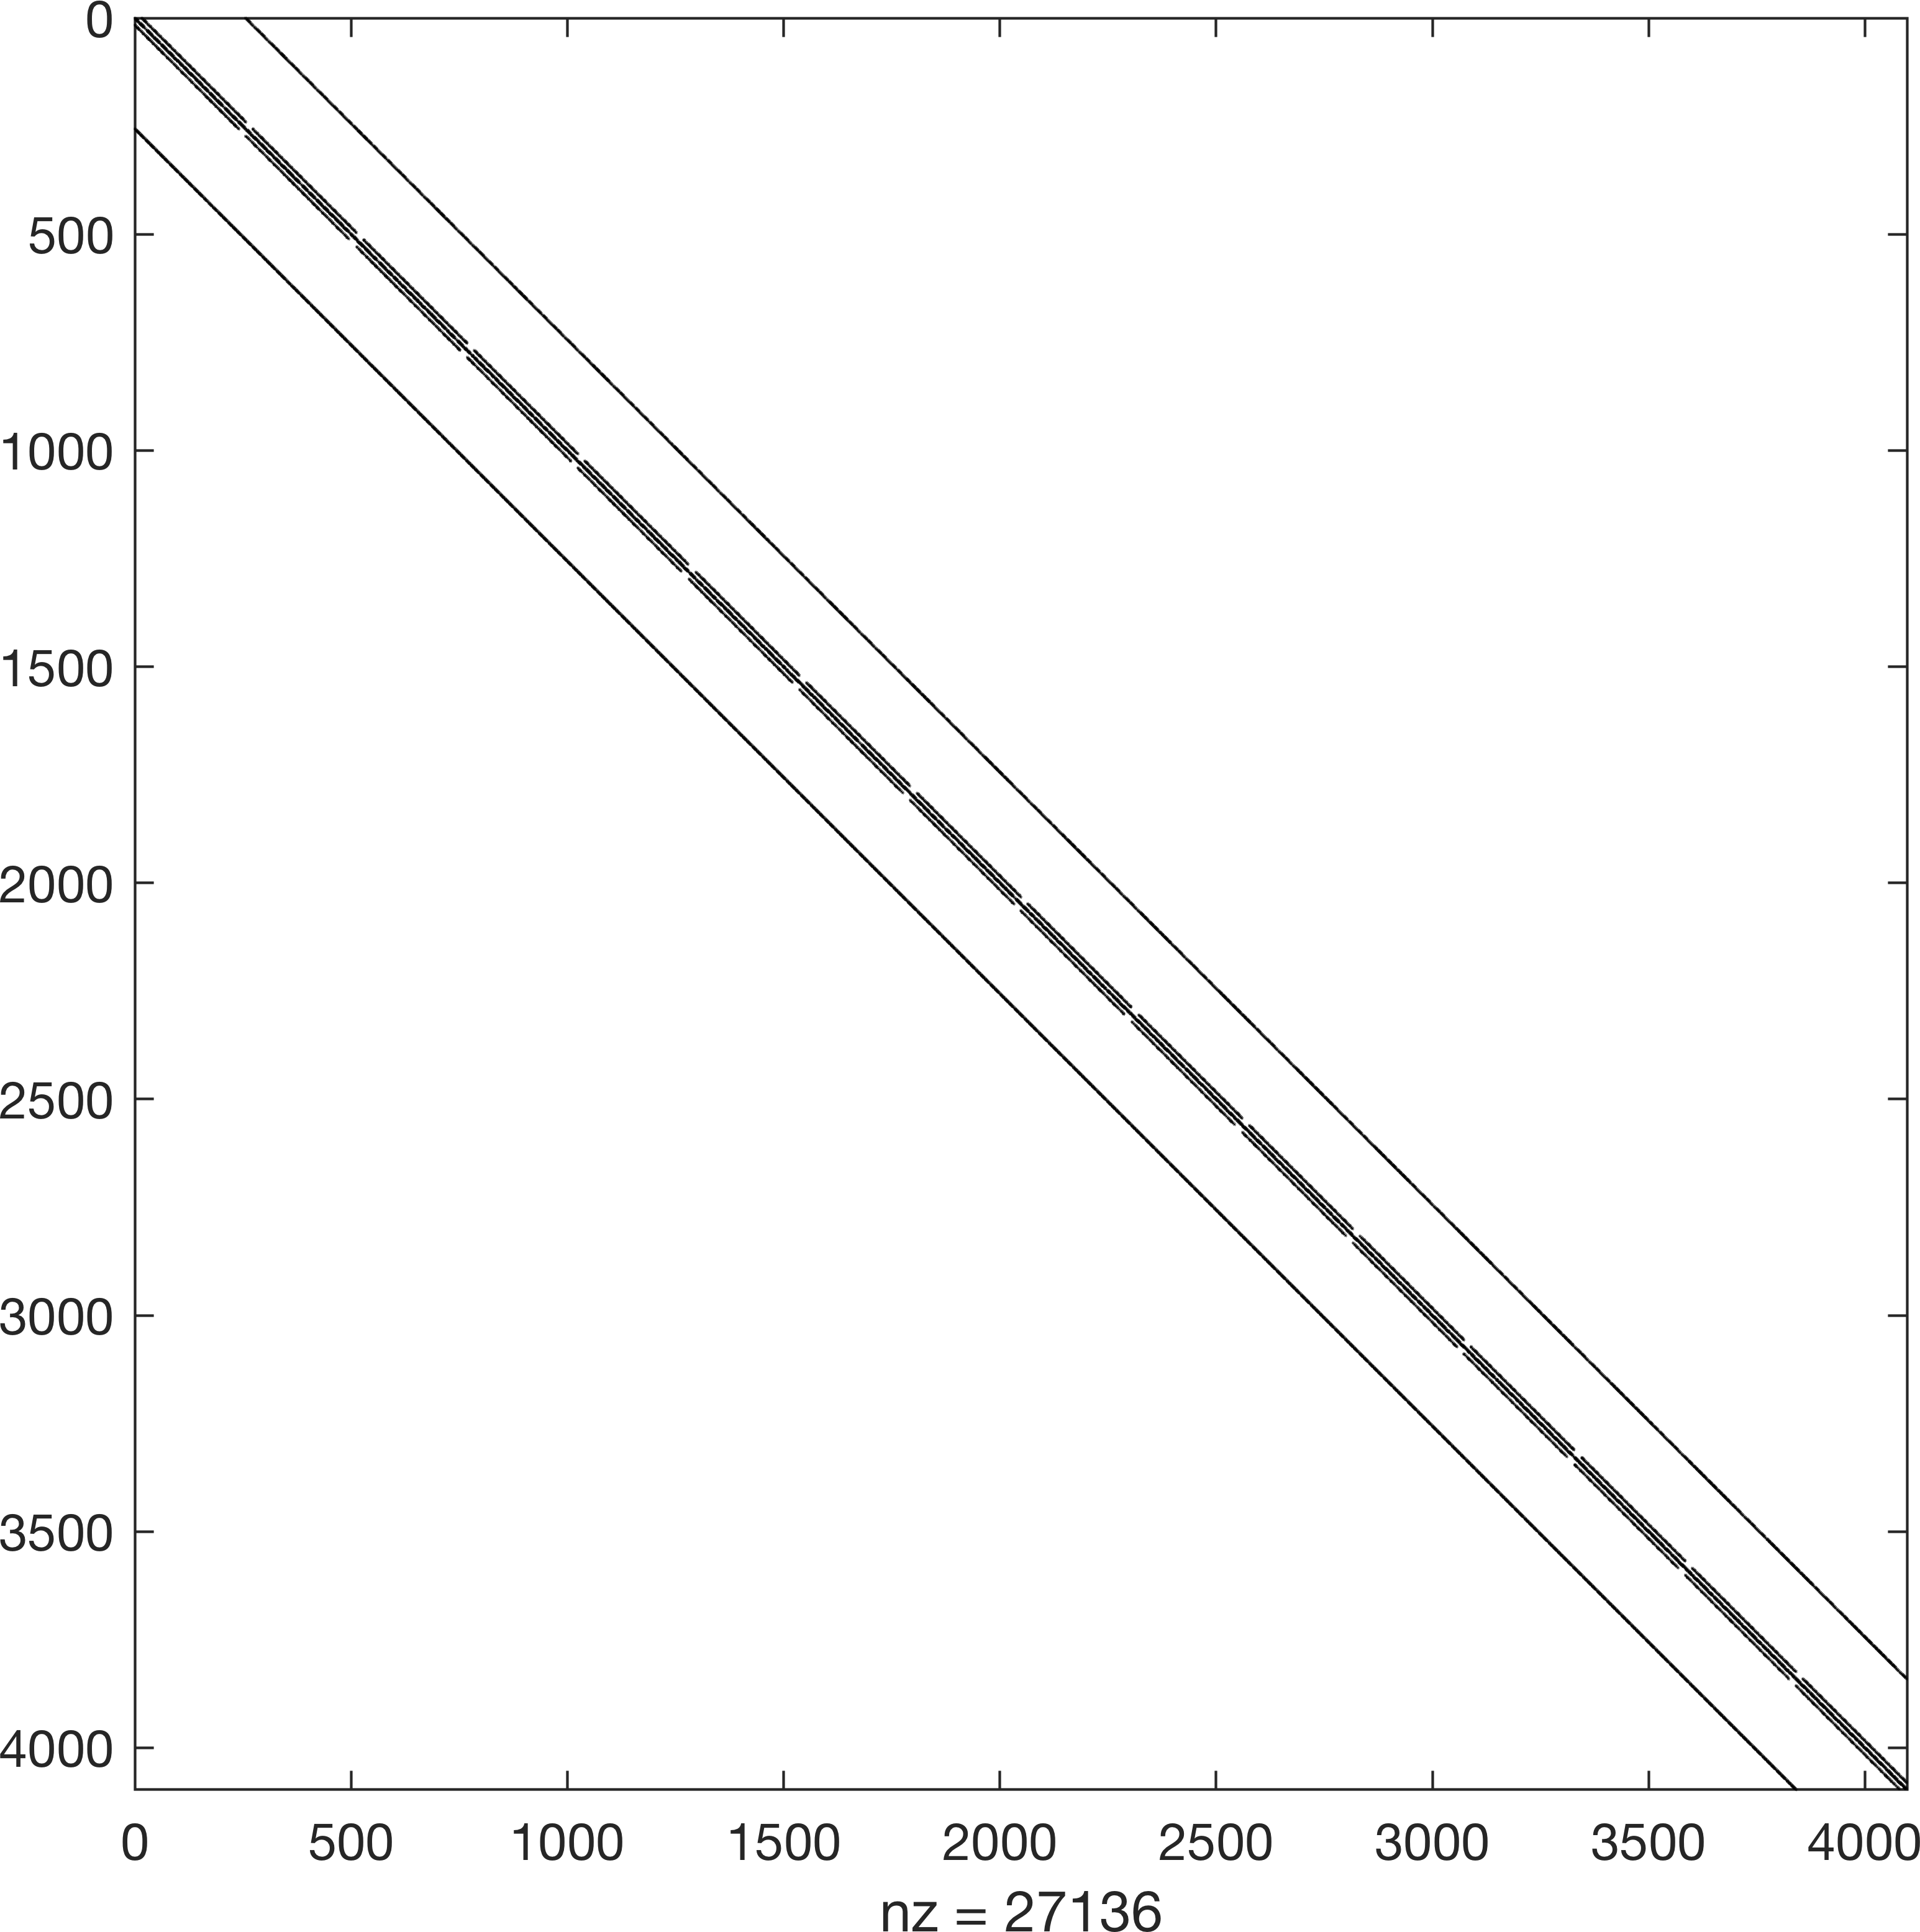
\includegraphics[width=0.32\textwidth]{\figPath/spy_A.png}\qquad\qquad\qquad
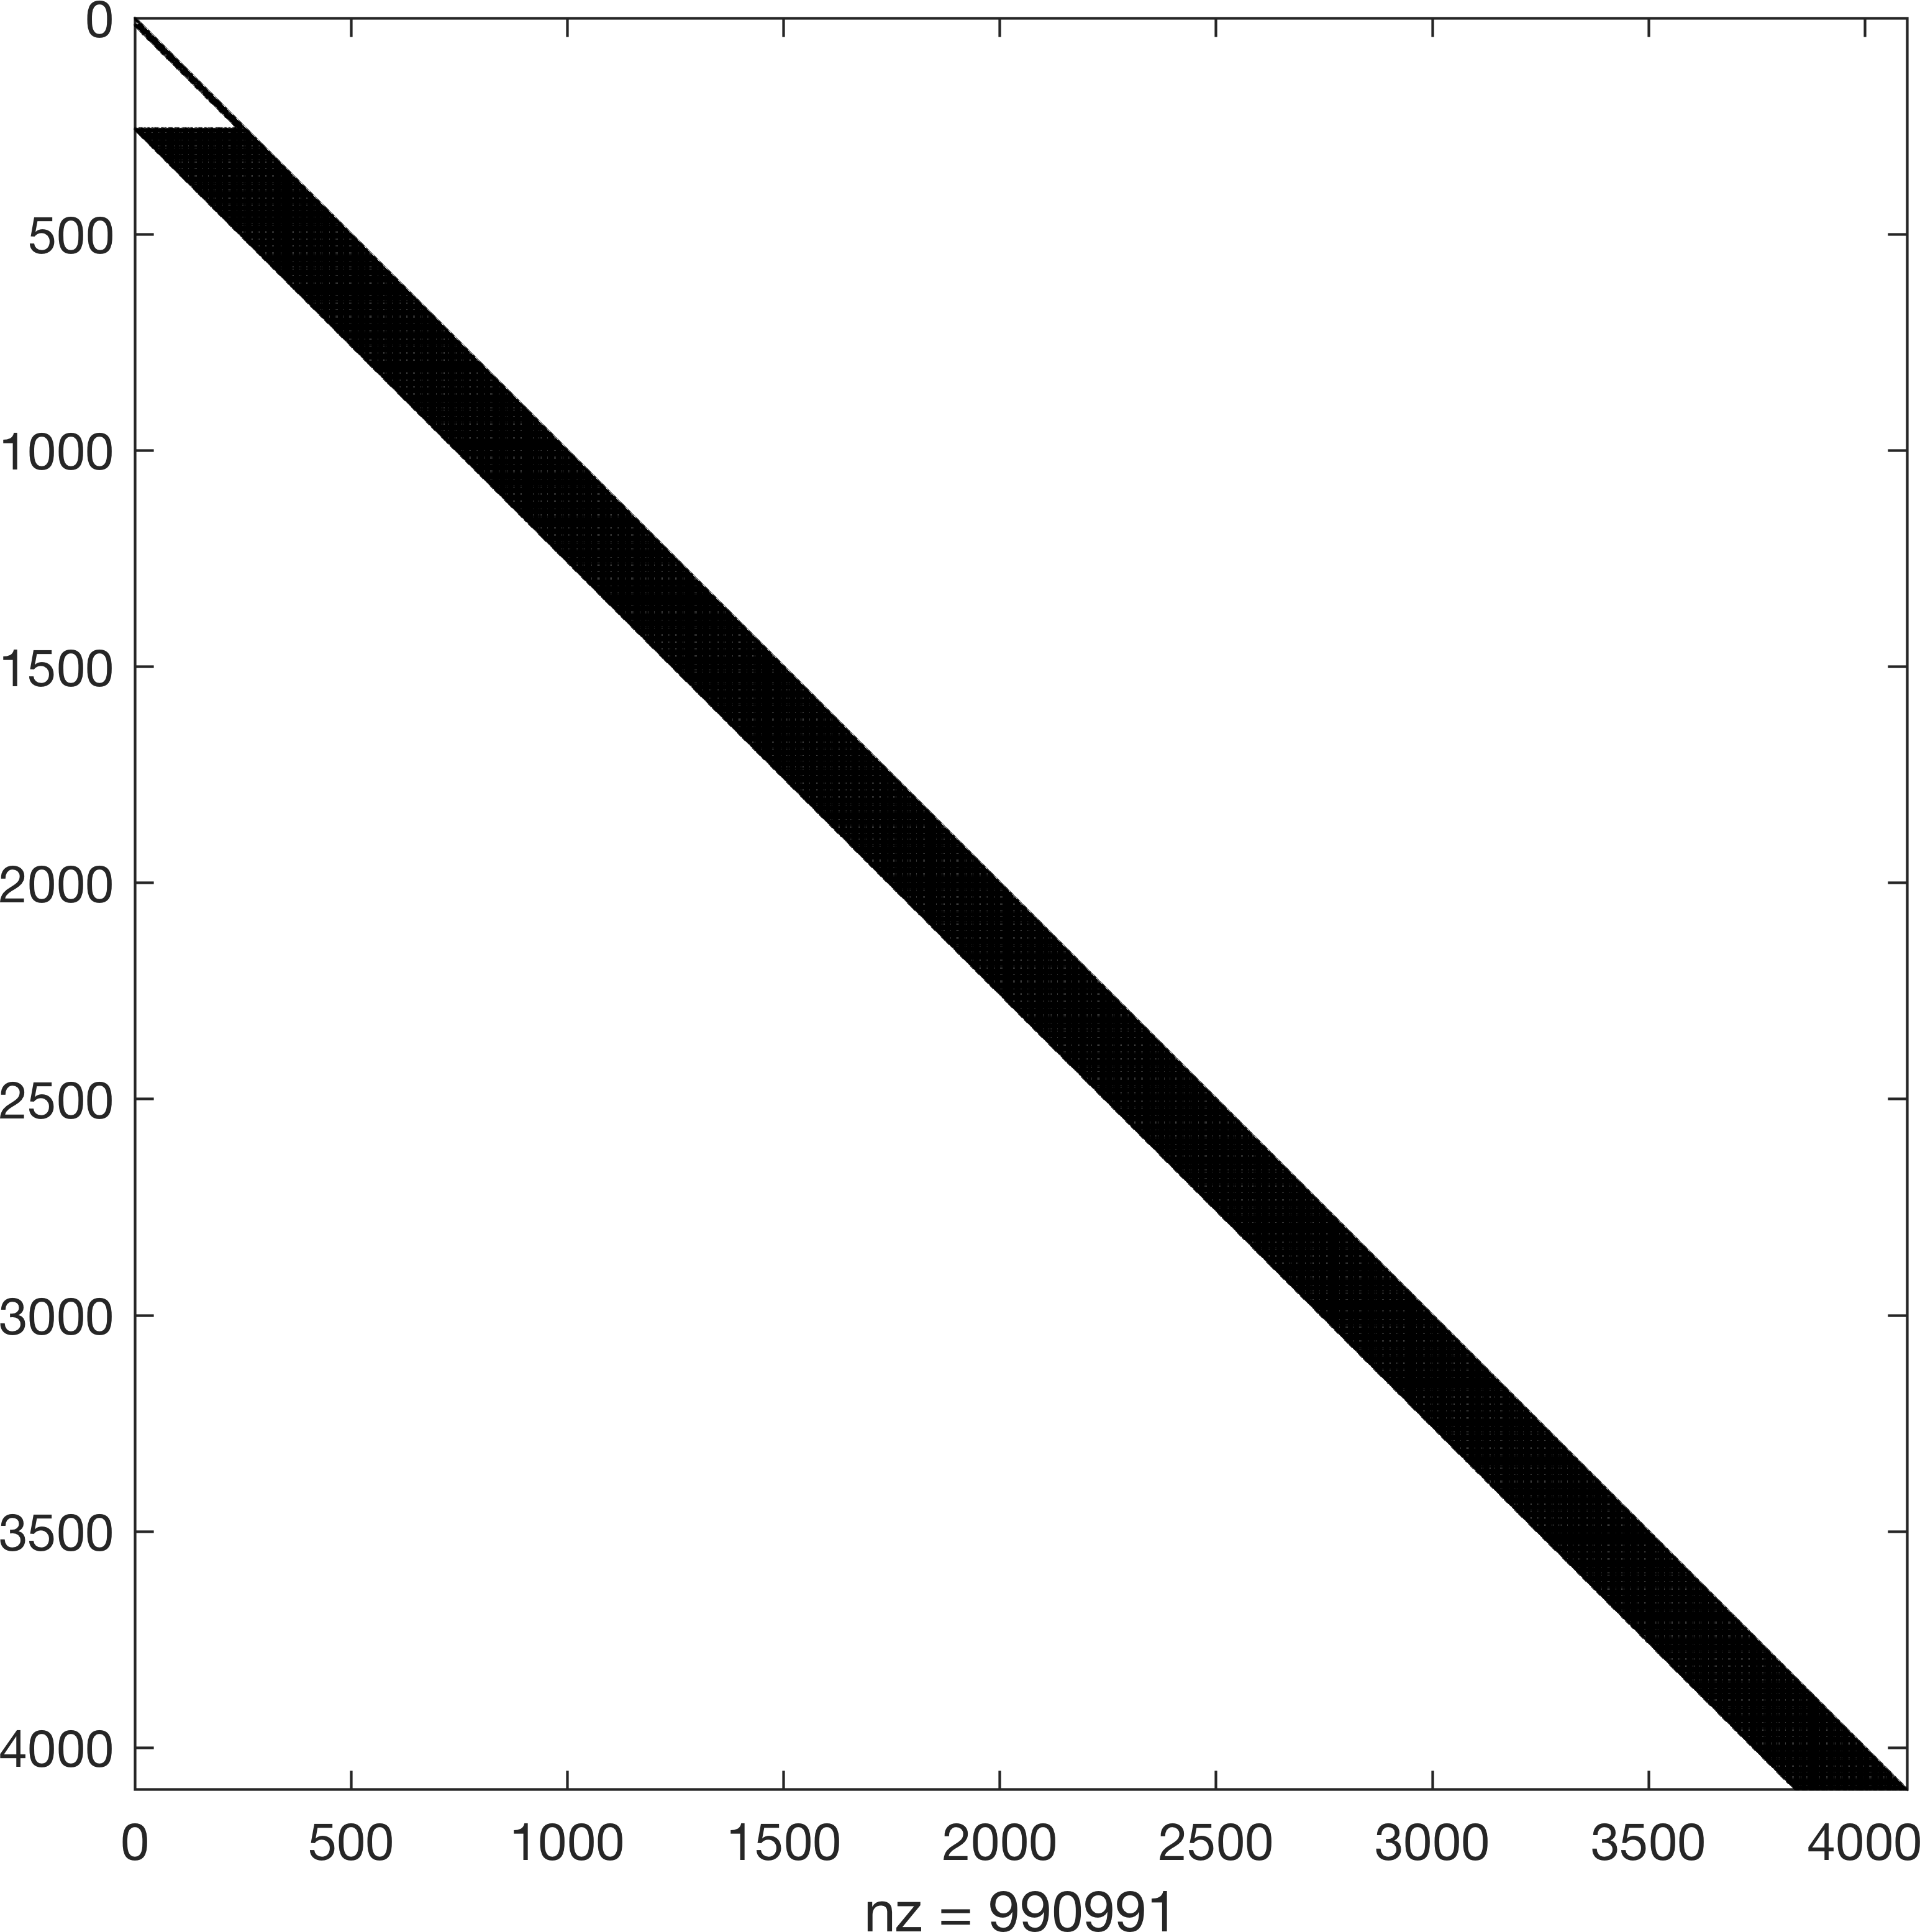
\includegraphics[width=0.32\textwidth]{\figPath/spy_L.png}\\
\end{center}
\caption[Sparsity patterns in case of a $LU$-decomposition for a refined 3D-cube with $16^3$ cells]{
Sparsity patterns in case of the $LU$-decomposition for a refined 3D-cube with $16^3$ cells.
(Left) Poisson matrix $A$ with about 27 thousand non-zeros; (Right) Lower triangular matrix $L$ with nearly 1 million non-zeros;
}
\label{FIG_SCARC_lu_memory_spy}
\end{figure}

The computing and storing of both triangular matrices can become prohibitively expensive, especially in case of huge systems of equations with many  millions of unknowns. This is true even if only the lower triangular matrix has to be stored for symmetric problems.
The example of the 3D-cube is taken up again in order to show the magnitudes of memory requirements to be expected here.
In case that the cube is refined from $16^3$ up to $128^3$ cells, Fig.~\ref{FIG_SCARC_lu_memory_need} compares
the number of non-zero entries of $L$ with those of $A$. Apparently the ratio dramatically deteriorates as the grid is refined. 
For the finest grid resolution of $128^3$ cells the matrix $L$ has about 2.18 billions %2,178,331,820 
of non-zeros whereas $A$ only has about 8.34 millions of non-zeros, %8,339,456 
corresponding to a ratio of about 238. Note, that for $A$ only its lower triangular and diagonal part must be stored due to its symmetry.

\begin{figure}[ht]
\centering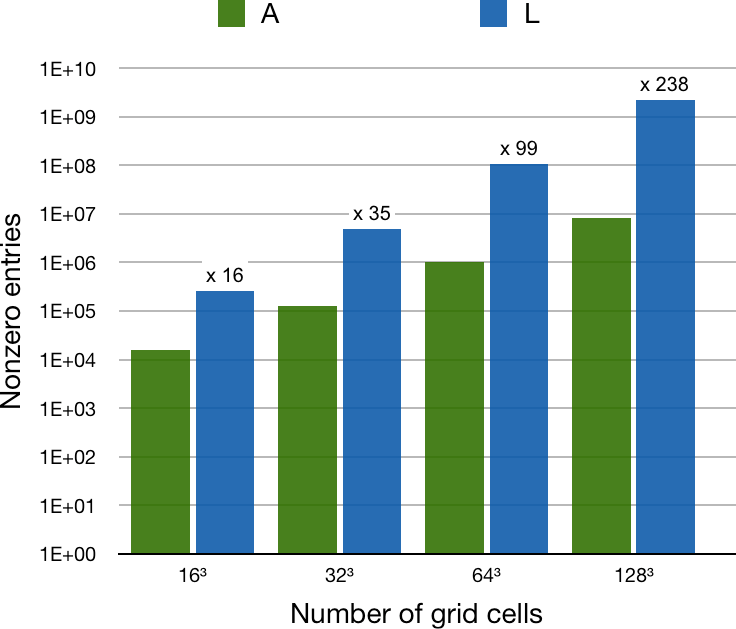
\includegraphics[width=0.5\textwidth]{\figPath/lu_memory_needs.png}\\[2ex]
\caption[Memory needs for the $LU$-decomposition]{
Number of non-zero entries in the Poisson matrix $A$ (green) and the lower triangular matrix $L$ (blue) of its $LU$-decomposition for different refinements of a 3D-cube from $16^3$ up to $128^3$ cells. The resulting ratio of $L$ to  $A$ is indicated at top of the blue bars. 
}
\label{FIG_SCARC_lu_memory_need}
\end{figure}

For realistically large CFD-problems the resulting additional storage requirements can  exceed the capacity of the available computing system in the worst case.
Thus, when considering the computational efficiency of $LU$-methods for a given application the resulting fill-in is a decisive criterion. 


% -----------------------------------------------------------------------------------------------------------------------------------
% Iterative solvers
% ------------------------------------------------------------------------------------------------------------------------------------
\subsection{Iterative solvers}
In contrast to direct solvers, iterative solvers perform multiple computational cycles producing a sequence of iterations which gradually improve an initial estimate of the solution until a predefined stopping criterion has been reached. 
%
Usually, they are easier to implement than direct ones, because they can be reduced to a series of core components such as matrix-vector multiplications, linear-combinations of vectors, scalar-products, etc.\ for which highly optimized program packages can be used, e.g.\ BLAS~\cite{Dongarra:2002}.
%
The computational complexity associated with each single cycle is comprehensively less compared to direct methods. Thus, the decisive question is how many cycles are needed for convergence.

Because iterative methods do not produce any fill-in, they preserve the sparsity structure of the system matrix and are much less demanding with respect to storage than direct methods.
%
However, iterative methods may depend on special properties of the underlying problem such as symmetry or positive-definiteness. Convergence can be very slow for ill-conditioned problems such that many iterations must be performed to reach the specified tolerance. Furthermore, they often require the optimal choice of certain algorithmic parameters which are highly problem-dependent and mostly difficult to predict a-priori.

% ------------------------------------------------------------------------------------------------------------------------------------------
% Basic iteration
% ------------------------------------------------------------------------------------------------------------------------------------------
\subsubsection{The basic iteration}
\label{SEC_SCARC_basic_iteration}
Based on Equation (\ref{EQ_SCARC_single_system}) the following simple relation applies
$ %\be 
%x = A^{-1} b = x -x + A^{-1} b = x - A^{-1} A x + A^{-1} b = x + A^{-1} (b-Ax)\,.
x = A^{-1} b = x + A^{-1} (b-Ax)\,.
$ %\ee
If the inverse $A^{-1}$ of the original system matrix $A$ is replaced by a suitable approximation matrix $B$ with $B \approx A^{-1}$
the so-called {\it preconditioned Richardson method}, or shorter, {\it basic iteration} for the solution of Equation (\ref{EQ_SCARC_single_system}) can be derived
\be 
  x^k = x^{k-1} + B\, (b - Ax^{k-1})\,. 
\label{EQ_SCARC_basic_iteration}
\ee
$x^k, x^{k-1} \in \mathbb{R}^{n}$ are iteration vectors and
$B \in \mathbb{R}^{n \times n}$ is a {\it preconditioning matrix} which can explicitly depend on an additional relaxation parameter $\omega\in \mathbb{R}$, that is, $B = B(\omega)$.

Equation (\ref{EQ_SCARC_basic_iteration}) is the typical core component of many iterative methods for the solution of Equation (\ref{EQ_SCARC_single_system}).
Starting with a initial guess $x^0$, it is used to successively minimize the {\it residual} or {\it defect}  $d^{k-1}:=b-A x^{k-1}$ which gives it also the name {\it defect correction method}.
Measured in a suitable norm the defect indicates how good the current iterate $x^k$ already fulfills equation $Ax=b$.
For the error $x-x^k$ in the $k$-th iteration step, there holds 
 \[ x-x^k = (I- B A)^k (x-x^0)\]
with the {\it error propagation operator} $F=(I- B \,A)$. The sequence of iterations $x^k$ converges to the solution of $Ax=b$ if and only if its {\it spectral radius}, the maximum of the absolute values of the eigenvalue, is smaller than 1. 

The convergence rate of iterative methods usually depends on the grid resolution, but can be comprehensively improved by appropriate selection of the preconditioning matrix $B$.
The goal behind is to transform the original system $Ax=b$  into an equivalent system $B\,Ax=B\,b$ whose solution requires significantly less iterations than that of the original system to satisfy a predefined termination criterion.
Or in other words, the transformed system $B\,Ax=B\,b$ should have a much better eigenvalue distribution than $Ax=b$ such that its condition number is substantially smaller and convergence can be reached much faster with less computational costs.

To achieve this goal, $B$ unfortunately has to meet two very contradictory conditions:
On the one hand, $B $ should be a good approximative inverse of $A$, i.e.\ $B \approx A^{-1}$, such that $B\,A$ is close to the identity matrix (with corresponding small condition number), but this means that $B$ is still very complex and expensive to use.
On the other hand, the application of $B$ should be much cheaper than the application of $A^{-1}$, i.e.\ $B \sim I$,  but that does not lead to an improvement at all. The more special properties of the original system $A$ can be incorporated into $B$, the better the convergence typically  is (i.e.\ the norm of the error propagation operator tends towards zero), but the higher the computational costs are, too. 
Again, a careful compromise has to be found.

\newpage
\paragraph{Preconditioning based on additive matrix splittings:}
For the definition of different preconditioners an additive 
splitting of $A$ into its diagonal part $D$, its lower triangular part $L$ and its upper triangular part $U$ can be used, i.e.\ $A=L + D+U$. Note, that for symmetric problems as the one considered here it holds $U=L$ which saves the additional storage of the upper matrix $U$.

Now, the simplest preconditioning is defined by using only the diagonal matrix, $B_{JAC} = D^{-1}$ ({\it Jacobi preconditioner}), which has the advantage that it can easily be inverted. But as expected this does not lead to any significant improvement of convergence speed. 
Involving more information of $A$ by also using its lower triangular part gives in a first step $B_{GS} = (L+D)^{-1}$ ({\it Gauss-Seidel preconditioner}) which is already much better but also more expensive to apply. Further improvements can be achieved by introducing an additional (optimal) relaxation parameter $\omega$ which leads to $B_{SOR} = (\omega L + D)^{-1}$  ({\it Successive Overrelaxation preconditioner}). For symmetric problems symmetrized versions of the preconditioners should be used accordingly. The preconditioner $B_{SSOR}$  ({\it Symmetric Successive Overrelaxation preconditioner}) combines two SOR passes, namely a forward pass followed by a backward pass traversing the cells in reverse order, such that the resulting preconditioning matrix is similar to a symmetric matrix. 
%$(D+\omegaL)^{-1}(D + \omega U)^{-1$\\
% $B_{SSOR}= (\frac{1}{2-\omega }(\frac{1}{\omega }D+L)(\frac{1}{\omega }D)^{-1}(\frac{1}{\omega }D+L)^{T})^{-1}$
%the matrix A is symmetric, then the Symmetric Successive Over-relaxation method, combines two SOR passes together in such a way that the resulting iteration matrix is similar to a symmetric matrix. Specifically, the first SOR sweep is carried out as in SOR, but in the second sweep the unknowns are updated in the reverse order. SSOR is a forward SOR sweep followed by a backward SOR sweep. The similarity of the SSOR iteration matrix to a symmetric matrix permits the application of SSOR as a pre-conditioner for other iterative schemes for symmetric matrices. Indeed, this is the primary motivation for SSOR since its convergence rate , with an optimal value, is usually slower than the convergence rate of SOR with an optimal value 
%M = (ω−1DA + LA)􏰀(2ω−1 − 1)DA􏰁−1(ω−1DA + UA)$
%A symmetric variant for the Gauss-Seidel preconditioner is defined by $B_{SGS}= ((D+L)D^{-1}(D+L)^{T})^{-1}$
%The Gauss-Seidel preconditioner is defined by
%M=L+D
%in which L is the strictly lower-triangular part of A and
%D = diag(A). By introducing a relaxation parameter, we get the SOR-preconditioner.
%For symmetric problems it is wise to take a symmetric preconditioner. %
%Only $O(n)$ operations required.

The dependence on the relaxation parameter $\omega$ can be very sensitive. An incorrectly chosen $\omega$ may quickly lead to divergence. Unfortunately,  its optimal value often depends on the refinement parameters and is a-priori difficult to determine.

Furthermore, the upper variants are mainly based on a very local way of proceeding: The iteration value in one single grid cell is computed as more or less simple mean value of its directly adjacent cells. New information can only be passed cell-by-cell through the whole domain which makes them unsuitable for problems with fast global data transport. Thus, they are rather bad solvers and in their pure form not suitable for complex problems. However, they have a decisive advantage which will give them further significance in the context of multigrid methods as will be explained below.

\paragraph{Preconditioning based on multiplicative matrix splittings:}
A more elaborate way of preconditioning is based on different multiplicative splittings of $A$. 
It was already described in Section \ref{SEC_SCARC_lu_decomposition} that the matrix can be decomposed into the product of a lower and upper triangular matrix $A=LU$, see again Fig.~\ref{FIG_SCARC_lu_decomposition}. Note, that in this case $L$ and $U$ are different from those in the additive decompositions above. 
If this factorization is used for preconditioning in case of a single-mesh application, $B_{LU}=LU$  ({\it $LU$-preconditioner}), the basic iteration will terminate within exactly one iteration because then $B=A$. If the system only needs to be solved once, nothing is gained from this procedure because the costs will remain the same as for the original system itself, or in other words, the system could have been solved by $LU$-decomposition from the beginning. 
%
But if the system has to be solved multiple times as is the case for FDS in the course of hundreds or thousands of time steps, it may be very advantageous to accept the costs for the factorization in an initial phase because in every subsequent time step the corresponding solution can be found by simple for- and backward substitution based on this decomposition which is computationally much cheaper. Note, that the multi-mesh case differs from this and will be treated separately again later.


However, the $LU$-decomposition is rather memory-intensive because it suffers from the undesired fill-in as already illustrated in Fig.~\ref{FIG_SCARC_lu_memory_need} above. For realistic 3D-problems this effect may be very pronounced. To remedy this situation, slimmed-down versions for the triangular matrices, $\tilde{L}$ and $\tilde{U}$, can be used alternatively. They are based on 
omitting entries smaller than a given tolerance or using the same (or a similar) pattern of non-zero elements as the matrix $A$ itself such that only the approximate relation $\tilde{L}\tilde{U}\approx A$ holds true. Thus, the resulting preconditioner, $B_{ILU} = \tilde{L}\tilde{U}$ ({\it ILU-preconditioner}), may be regarded as an incomplete, but computationally much cheaper variant of its complete counterpart. 
Unfortunately, $ILU$-preconditioning is not always stable. But it has proven to be rather efficient in many fields of application if the most basic information of $A$ can be incorporated. Its application as preconditioner in FDS will be tested in medium term as well.

Finally, the mesh-wise preconditioning can also be performed by means of local FFT methods, provided that a structured discretization is used. As the later test calculations will show, among the variants considered here so far, this turns out to be the fastest type of mesh-wise preconditioning for structured applications of the basic iteration and its later generalizations. 

% ------------------------------------------------------------------------------------------------------------------------------------------
% Preconditioning based on domain decomposition
% ------------------------------------------------------------------------------------------------------------------------------------------
\paragraph{Preconditioning based on domain decomposition:}
\label{SEC_SCARC_block_precon}

In the course of a domain decomposition method the computational domain $\Omega$ is subdivided into single subdomains $\Omega_i$, i.e.\ 
$\Omega=\cup_{i=1, \dots, M} \,\Omega_i\,$. Now, the individual operations of the basic iteration must be performed in a distributed manner.
%
To this end, let $K$ be the set of all cells in $\Omega$ and $K_i \subset K$ the subset of cells belonging to subdomain $\Omega_i$, such that $K=\cup_{i=1, \dots, M}\, K_i$.
The number of cells in $\Omega$ and $\Omega_i$ are defined by $n := \mid\!\! K \!\!\mid$ 
and $n_i := \mid\!\! K_i \!\!\mid$, respectively.

On every subdomain $\Omega_i$ the local coefficient matrix $A_i \in \mathbb{R}^{n_i \times n_i}$ is
then defined as a restriction of the global matrix $A \in \mathbb{R}^{n \times n}$ to the
set $K_i$.  %spoken intuitively ``$\,A_i \equiv \restrict{A}{\Omega_i}$''.
%
Its formal algebraic definition requires a {\it prolongation matrix} $R_i^T \in \mathbb{R}^{n \times n_i}$ which
positions a local vector $x_i \in \mathbb{R}^{n_i}$ from subdomain $\Omega_i$ 
to the corresponding positions of the global vector $x \in \mathbb{R}^n$ in the global domain $\Omega$,% and replaces the missing parts with zeros:
\[
(R_i^T x_i)_j :=
 \left\{
  \begin{array}{l@{\,, \quad }l}
   (x_i)_j & \mbox{if $j \in K_i  \,,$} \\[1.2ex]
   0       & \mbox{if $j \in K-K_i\,.$} 
  \end{array}
 \right.
\]
Vice versa, the transposed {\it restriction matrix} $R_i \in \R^{n_i \times n}$ restricts a global vector $x\in \R^n$ to its local counterpart $x_i \in \R^{n_i}$ by only chosing the corresponding entries from $K_i$.  
Thus, the local matrices are defined by
\be
A_i := R_i A R_i^T\,, \qquad i=1, \ldots, M\,,
\label{EQ_SCARC_subdomain_matrices}
\ee
and respresent $n_i \!\times\! n_i$-sized sub-blocks of $A$. Special properties of $A$ (as e.g.\ diagonal dominance and positive definitness) are preserved. Note, that the matrices $R_i$ und $R_i^T$ are never explicitly built but are only defined by their action.

Now, most of the core components of the basic iteration (\ref{EQ_SCARC_basic_iteration}) can simply be computed in a data-parallel way.
Matrix-vector multiplications $Ax$, as needed for the defect computation, are computed in two steps: First, only the sub-mesh-related local matrix-vector products $y_i$ are computed simultaneously.
Secondly, these local contributions are combined to a global matrix-vector product $y$ using the upper prolongation operators, 
\be 
y = A\, x = {\widetilde{\sum}}_{i=1, \ldots, M}\, R_i^T y_i = {\widetilde{\sum}}_{i=1, \ldots, M}\, R_i^T A_i x_i\,.
\label{EQ_SCARC_matvec_product}
\ee
Here, the corresponding entries at inner boundary cells require a special treatment: As illustrated in Fig.~
\ref{FIG_SCARC_matvec_exchange}, a matrix stencil that is positioned at an inner boundary cell has one or more `legs' that reach out of the subdomain into its direct neighbors, but the related values of $x$ which are needed for the sum in Equation (\ref{EQ_SCARC_matvec_product}) are initially missing there. To guarantee that the same final matrix-vector product is achieved as for a corresponding serial execution, these values must be exchanged via  next-neighbor communication which is indicated by the marked sigma sign in Equation (\ref{EQ_SCARC_matvec_product}).

\begin{figure}[ht]
\scalebox{1.0}{
\begin{minipage}[t]{1.0\textwidth}
\begin{center}
\begin{tikzpicture}
[
scale=0.75,
every node/.style ={scale=0.75},
inner sep=1mm,
%scale=1.0,
L2A/.style={circle, draw=black!40, fill=blue!10, thin, minimum size=7.5mm},
L1/.style={rectangle, draw=black!40, fill=black!03,   thin, minimum size=6cm},
box/.style = {very thin, black!70, rectangle, inner xsep=10pt, inner ysep=10pt,},
inner sep=0.6mm,
],
%
% \draw [L1] (0.25,2) -- (7.5,2);
\fill [black!4] (0.5,0.5) rectangle (4,2.0);
\fill [black!8] (4.0,0.5) rectangle (7.5,2.0);
\fill [black!6] (0.5,2.0) rectangle (4,8.5);
\fill [black!2] (4.0,2.0) rectangle (7.5,8.5);

\draw [step=1.0, very thin, black!20] (0.5,0.5) grid (7.5,8.5);
\draw [very thick] (0.5,2) -- (7.5,2);
\draw [very thick] (4,0.5) -- (4,8.5);

\node at (8.3, 4.5)  {\LARGE \,$\cdot \,\frac{1}{h^2}$};

\node [L2A]  (M1)   at ( 4.5, 2.5)  {$-4$};
\node [L2A]  (S1)    at ( 4.5, 1.5)  {$1$};
\node [L2A]  (W1)   at ( 3.5, 2.5)  {$1$};
\node [L2A]  (E1)    at ( 5.5, 2.5)  {$1$};
\node [L2A]  (N1)    at ( 4.5, 3.5)  {$1$};
%
\draw [thick]  (M1.south)  -- (S1.north) ;
\draw [thick]  (M1.west) -- (W1.east) ;
\draw [thick]  (M1.north) -- (N1.south) ;
\draw [thick]  (M1.east) -- (E1.west) ;
%
\node [L2A]  (M2)   at ( 3.5, 6.5)  {$-4$};
\node [L2A]  (S2)    at ( 3.5, 5.5)  {$1$};
\node [L2A]  (W2)   at ( 2.5, 6.5)  {$1$};
\node [L2A]  (E2)    at ( 4.5, 6.5)  {$1$};
\node [L2A]  (N2)    at ( 3.5, 7.5)  {$1$};
%
\draw [thick]  (M2.south)  -- (S2.north) ;
\draw [thick]  (M2.west) -- (W2.east) ;
\draw [thick]  (M2.north) -- (N2.south) ;
\draw [thick]  (M2.east) -- (E2.west) ;

\node [box] (box) at (1.5,1.0){Mesh3};
\node [box] (box) at (6.5,1.0){Mesh4};
\node [box] (box) at (1.5,8.0){Mesh1};
\node [box] (box) at (6.5,8.0){Mesh2};

%
\end{tikzpicture}

\caption{The computation of global matrix-vector products requires next-neighbor communications along mesh interfaces since in an internal boundary cell single legs of the corresponding matrix stencil may reach into a neighboring mesh.}
\label{FIG_SCARC_matvec_exchange}
\end{center}
\end{minipage}}
\end{figure}

Since the spatial discretization for the pressure is based on cell midpoints, linear combinations, $\alpha x+ \beta y$, of vectors $x$ and $y$ do not require any communication at all. Every subdomain simply holds its associated part of the global vector, but along mesh interfaces no redundancies can occur. Thus, fundamental parts of the basic iteration can be done simultaneously and continue to operate globally in the same way as a hypothetic serial computation.

%This matrix is just the same matrix which you would get if you discretized the complete geometry within ONE big grid. 

The situation is more complicated for the various preconditioners. %which differ more or less comprehensively from their serial counterparts.
With a view to the underlying domain decomposition, a natural strategy is to break up the preconditioning according to the domain decomposition. Now, each subdomain applies its own preconditioning based on approximations for the local matrix inverses $A_i^{-1}$. 
For example, the block-wise analogue of the Jacobi preconditioner looks like
\[ x^k = x^{k-1} + \sum_{i=1}^M R_i^T D_i^{-1} R_i\, (b - Ax^{k-1})\,, \]
where each subdomain only uses the local diagonal matrix $D_i$ for preconditioning.
The solution of the local preconditioning problems only incorporates purely local computations which can be performed simultaneously with maximum possible exploitation of the local processor power. Their final global coupling only requires local next-neighbor communication. 
Thus, the resulting {\it block-preconditioning} yields significant improvements in the parallel efficiency. 

However, as already explained, this strategy is associated with a breakup of the strongly recursive dependencies of optimal serial preconditioners such that numerical efficiency may strongly deteriorate in terms of poorer convergence rates compared to the serial analogues and also dependencies on the number of subdomains and/or other refinement parameters. Besides, the efficiency of the block-preconditioning can be difficult to predict for realistic geometries with complex combinations of the single subdomains.
%
More details about preconditioning based on domain decomposition techniques will be given in the subsequent Section (\ref{SEC_SCARC_scarc}). 

\newpage
% ------------------------------------------------------------------------------------------------------------------------------------------
% Generalizations of the basic iteration
% ------------------------------------------------------------------------------------------------------------------------------------------
\subsection{Efficient Generalizations of the Basic Iteration}
\label{SEC_SCARC_generalizations}
Even for powerful preconditioners the  basic iteration (\ref{EQ_SCARC_basic_iteration}) is rather inefficient and requires a comprehensible number of iterations to drive the solution within a predefined tolerance. This especially holds true for complex situations with complicated geometric details.
But the single representatives can be embedded into much stronger generalized schemes such as the global {\it preconditioned conjugate gradient method} (CG) or a {\it geometric multigrid method} (MG).
Both schemes are closely related, because they are based on simple defect
correction iterations, which approximate the error by using a sequence of smaller subproblems. 
The main difference between both is found in the choice of the underlying subspaces.
A brief overview of both classes is given below.
%This issue is discussed in more detail in 
%??. %\mcite{Hackbusch }\cite{Hackbusch94}. 


% ------------------------------------------------------------------------------------------------------------------------------------------
% Preconditioned conjugate gradient method
% ------------------------------------------------------------------------------------------------------------------------------------------
\subsubsection{Preconditioned Conjugate Gradient Method}
\label{SEC_SCARC_cg}

CG-methods belong to the class of {\it Krylov subspace} methods which iteratively construct a $k$-dimensional vector space, 
$\mbox{span}\{r,Ar,...,A^{k-1}r\}$, using A-orthogonalisation. They are designed to find the minimum of the quadratic form $F(x)=1/2\, x^T A x - x^T b \rightarrow 0$ which is equivalent to solving Equation (\ref{EQ_SCARC_single_system}). 
New search directions are constructed in such a way that they are orthogonal to all previous residuals and search directions. This process guarantees a steady improvement of the search directions and convergence to the minimum of the quadratic form after at most $n$ steps. %This subspace is called a Krylov subspace, a subspace created by repeatedly applying a matrix to a vector. 
%TOFIX: The Krylov subspace is the $m$-dimensional vector space span{r(0),Ar(0),...,Am−1r(0)}. All Krylov subspace methods iteratively construct such a vector space based on A-orthogonalisation.

Below a general algorithmic description of the CG-method for the solution of Equation (\ref{EQ_SCARC_single_system}) with preconditioning by $B$ is given.
Therein, the notation $(v,w)=v^T w$ denotes the standard scalar product of two vectors with the corresponding norm $\|v\| =\sqrt{(v,v)}$.
Using the 2D pipe geometry of Figure \ref{FIG_SCARC_basic_pipe_geometry}, the CG method is also graphically represented in Figure \ref{FIG_SCARC_cg_method}.

\paragraph{\underline{Conjugate gradient method for the solution of $Ax=b$ with preconditioning by {\boldmath {$B$}}}} \mbox{} \\[1ex]
Given an initial guess $x^0$, then perform the following steps: \\[2ex]
\begin{tabular}{ccll}
%
\multicolumn{1}{l}{\bf Initialization:}&&&\\[1ex]
\hspace{1.0cm} $r^0$ & $\hspace{0.2cm}=$ & $A x^0-b$      & \hspace{1.0cm} initial residual $x^0$      \\[1.0ex]
\hspace{1.0cm} $v^0$ & $\hspace{0.2cm}=$ & $B\,\, r^0$  & \hspace{1.0cm} preconditioning  \\[1.0ex]
\hspace{1.0cm} $d^0$     & $\hspace{0.2cm}=$ & $-v^0$          & \hspace{1.0cm} vector update 	     \\[2.0ex]
%
 \multicolumn{1}{l}{\bf Iteration \boldmath $k\geq 0$:}&&&\\[1ex]
\hspace{1.0cm}$\alpha_k$ & $=$ & $(r^k, v^k)/(d^k, A d^k)$     & \hspace{1.0cm} new search parameter		     \\[1.0ex]
\hspace{1.0cm}$x^{k+1}$     & $=$ & $x^k + \alpha_k \,d^k$          & \hspace{1.0cm} new solution	   \\[1.0ex]
\hspace{1.0cm}$r^{k+1}$  & $=$ & $r^k + \alpha_k \,A d^k$      & \hspace{1.0cm} new residual		     \\[1.0ex]
\hspace{1.0cm}$v^{k+1}$  & $=$ & ${B\,\, r^{k+1}}$        & \hspace{1.0cm} preconditioning     \\[1.0ex]
\hspace{1.0cm}$\beta_k$  & $=$ & $(r^{k+1}, v^{k+1})/(r^k,v^k)$   & \hspace{1.0cm} new search parameter	  \\[1.0ex]
\hspace{1.0cm}$d^{k+1}$  & $=$ & $- v^{k+1} + \beta_k d^k$      &\hspace{1.0cm} new search direction    \\[1.0ex]
\hspace{1.0cm}$\| r^{k+1}/r^0 \|$ & < &$\epsilon$ 			& \hspace{1.0cm} convergence check			\\[1.5ex]
\end{tabular}

\begin{figure}[ht]
\begin{center}
\begin{tikzpicture}
[
scale=0.6,
every node/.style={scale=0.6},
Background/.style={rectangle,draw=black!04,fill=black!04, thin, minimum size = 4 cm},
Obstruction/.style={rectangle,draw=black!70,fill=black!40, very thick, minimum size=1cm},
GlobalBorder/.style={-.,draw=black!100,  thin},
Finegrid/.style={step=0.5cm,gray,very thin},
Thickline/.style={-,draw=black!100,fill=black!02, very thick},
Thinline/.style={draw=black!100,fill=black!02, very thin},
Ball/.style={circle, draw=black!40, fill=red!20, thin, minimum size=3.5mm},
Circle/.style={circle,draw=black!40,fill=black!06,thin,minimum size=35.5mm},
Rectangle/.style={rectangle,draw=black!10,fill=white,inner xsep=0pt, inner ysep=0pt,},
Box/.style= {very thin, rectangle, inner xsep=10pt, inner ysep=10pt,},
DotBox/.style= {very thick, rectangle, inner xsep=0pt, inner ysep=8pt, dotted, fill=white, draw=black!70,},
ComRedArrow/.style= {very thick, draw=red!70,},
ComBlueArrow/.style= {very thick, draw=blue!70,},
DotArrow/.style= {<-, thick, dotted, draw=black!70,},
DotLine/.style= {very thick, dotted, draw=black!70,},
]

%\draw[GlobalBorder, fill=black!10] (-1.2,-1.2)--(13.2,-1.2)--(13.2,9.2)--(-1.2,9.2)--(-1.2,-1.2);
\node [Box, black] (box) at (8.0,8.7){\LARGE Global CG-method};

\node[Background] at (  2,2) {};
\node[Background] at (  6,2) {};
\node[Background] at (  6,6) {};
\node[Background] at (10,6) {};

\node[Obstruction] at (2,2) {};

\draw[Finegrid] (0,0) grid (  8,4);
\draw[Finegrid] (4,4) grid (12,8);

\draw[Thickline] (0,0)--(  8,0);
\draw[Thickline] (4,8)--(12,8);
\draw[Thickline] (0,4)--(  4,4);
\draw[Thickline] (8,4)--(12,4);

\draw[Thickline] (  0,0)--(  0,4);
\draw[Thickline] (  4,8)--(12,8);
\draw[Thickline] (  4,4)--(  4,8);
\draw[Thickline] (  8,0)--(  8,4);
\draw[Thickline] (12,4)--(12,8);

\draw[Thickline] (4,0)--(4,4);
\draw[Thickline] (4,4)--(8,4);
\draw[Thickline] (8,4)--(8,8);

\node[Rectangle] at (  2,2.0) {\Large \begin{tabular}{c} Local \\ Precon\end{tabular}};
\node[Rectangle] at (  6,2.0) {\Large \begin{tabular}{c} Local \\ Precon\end{tabular}};
\node[Rectangle] at (  6,6.0) {\Large \begin{tabular}{c} Local \\ Precon\end{tabular}};
\node[Rectangle] at (10,6.0) {\Large \begin{tabular}{c} Local \\ Precon\end{tabular}};

\draw[<->,ComRedArrow](3.2,1.75)--(4.8,1.75);
\draw[<->,ComRedArrow](5.75,3.2)--(5.75,4.8);
\draw[<->,ComRedArrow](7.2,5.75)--(8.8,5.75);

\draw[<->,ComBlueArrow](3.2,2.25)--(4.8,2.25);
\draw[<->,ComBlueArrow](6.25,3.2)--(6.25,4.8);
\draw[<->,ComBlueArrow](7.2,6.25)--(8.8,6.25);

\draw[<-, ComBlueArrow](3.25,3.25)--(4.75,3.25);
\draw[->, ComBlueArrow](4.75,3.25)--(4.75,4.75);
\draw[<-, ComBlueArrow](7.25,3.25)--(8.75,3.25);
\draw[->, ComBlueArrow](8.75,3.25)--(8.75,4.75);
\draw[<-, ComBlueArrow](3.25,0.75)--(10,0.75);
\draw[->, ComBlueArrow](10.0,0.75)--(10,4.75);

\draw[<->,ComRedArrow](-4.8,7.0)--(-3.2,7.0);
\node [Box,red!70] (box) at (-0.0,7.0){%
    \begin{minipage}{0.56\textwidth}
    \begin{center}
        {\Large Local communication}
    \end{center}
    \end{minipage}};
    
\draw[<->,ComBlueArrow](-4.8,5.8)--(-3.2,5.8);
\node [Box,blue!70] (box) at (-0.0,5.8){%
    \begin{minipage}{0.56\textwidth}
    \begin{center}
        {\Large Global communication}
    \end{center}
    \end{minipage}};
    

\end{tikzpicture}

\caption{Data-parallel global CG-method with mesh-wise preconditioning for the 2D pipe geometry. Local communication is needed for matrix-vector products, global communication for scalar products and defect norms.} 
\label{FIG_SCARC_cg_method}
\end{center}
\end{figure}

Standard methods are restricted to symmetric positive-definite problems, but
there also exist variants for the non-symmetric case, the so-called {\it BICG-methods} see e.g.~\cite{Saad:2003} or~\cite{Axelsson:1998}.
%
They only need less storage space for several auxiliary vectors and are largely based on matrix-vector multiplications and global scalar-products.
In the multi-mesh case, most operations can be performed in a purely data-parallel way: All matrix vector products, linear combinations, norms and scalar products give the same results as for a hypothetic single-mesh execution, but are only calculated in a distributed manner which is indicated by the only dashed boundaries between the single sub-meshes. For matrix-vector products this requires the (computationally cheap) local data exchanges between directly adjacent meshes as already described. For global scalar products %, i.e.\ $s=\lsumiN s_i = \lsumiN(v_i,w_i)$, 
and global norms, respectively, the local contributions must be exchanged between all meshes to finally get a global sum. Certainly, this leads to a worsening of the parallel efficiency because the processors have to synchronize and possibly wait for each other which has a negative effect especially in geometric complex cases where the meshes cannot be evenly distributed among the processors. On the other hand, these global operations also contribute to much stronger global coupling.

Typically, the convergence rate of CG-methods  depends on the discretization parameters, but can be considerably improved by choosing a suitable preconditioning matrix $B$. For its construction, domain decomposition techniques can be used effectively, see~\cite{Bramble:1991}.
There exists an upper bound for the required number of iterations which is
proportional to the square root of the {\it condition number} $\kappa (B \, A) = \lambda_{max} (B \, A) / \lambda_{min} (B\, A)$,
\[ \| e_k \|_A \leq 2 \big(\frac{\sqrt{\kappa (B \,A)} -1}{\sqrt{\kappa (B \,A)} +1}\big)^k \| e_0\|_A\,\]  
Here, $\lambda_{min}$ and $\lambda_{max}$ denote the smallest/biggest eigenvalue of $B A$, $e_k= x_k - x$ the error between the iterative solution $x_k$ and the exact solution $x$, and  $\|x\|_A := (Ax,x) ^{1/2}$ the corresponding $A$-norm.

The acceleration of convergence by reducing the condition number of the preconditioned system $\kappa(B \, A)$ compared to that of the original system $\kappa(A)$ should at least compensate for the extra cost of computing the product $B r^{k+1}$ in the upper algorithm, 
but in the best case, of course, be much larger. 
%
Geometrically, the idea behind the preconditioning in CG-methods can be understood as a transformation of the quadratic form into a more spherical shape such that the eigenvalues are closer together. While the simple diagonal Jacobi-preconditioning matrix $D$ only scales along the coordinate axes, the perfect preconditioner $B=A$ performs a scaling along the eigenvector axes leading to the optimal possible effect $\lambda_{max}=\lambda_{min}$ with a resulting condition number of one.



The ultimate goal is to construct an optimal
preconditioner with a convergence rate independent of the fine grid resolution, the size of the sub-meshes (or their number respectively) and also of possibly present anisotropies. In practise, this goal is usually hard to achieve and strongly depends on the individual situation. Nevertheless, there are many possibilities, especially on the basis of  domain decomposition techniques, to achieve a more or less pronounced improvements.% which will be presented below.

% ------------------------------------------------------------------------------------------------------------------------------------------
% Geometric multigrid method
% ------------------------------------------------------------------------------------------------------------------------------------------
\subsubsection{Geometric Multigrid Methods}
\label{SEC_SCARC_mg}

Fast convergence rates independent of the grid size with moderate computational complexity may be reached with MG-methods. The term `multigrid' should not be confused with the term `subdomain': It does not refer to a sequence of different sub-grids arising from a domain decomposition but rather a hierarchy of grids with different resolutions for one and the same mesh.
MG-methods act on a hierarchy of grids with different resolutions and are able to achieve fast convergence rates independent of the grid size with moderate computational complexity.

The basic idea behind MG-methods is to improve the convergence speed of the basic iteration by correcting the defects on successively coarser grids.
This process explicitly uses an important property of the single representatives of the basic iteration, namely the so called {\it smoothing property}: As can be shown by a Fourier analysis, the high-frequency error components are damped out very quickly, often in only a few iterations, whereas the low-frequency error components are very persistent towards additional iterations.
This special property is based on the fact that the new iteration value in a single grid point is computed as more or less simple mean value of the surrounding grid values. If this set of nodes is already smoothed out, hardly any further improvement can be achieved. Thus, new information is only propagated very slowly through the whole domain. Informally, the whole multigrid procedure looks like this:

\begin{itemize}
\item {\bf Pre-Smoothing:}
Starting from a given initial solution on the finest grid level, several steps of a simple basic iteration with a suitable matrix $B$ are performed. After only a few iterations 
the mentioned smoothing property usually leads to a considerable reduction of the high-frequent error components of the defect while the low-frequent components are nearly unchanged and still may be very large. 
This suggests to restrict this  {\it smoothed}  defect  on the next coarser grid (e.g.\ with the double grid size) by using a suitable grid transfer operator based on interpolation, where it can be approximated at much lower costs. 
\item {\bf Coarse grid correction:} The alternating interplay of smoothing and restriction
may be continued until the coarsest grid level has been reached where the remaining coarse grid problem can be solved exactly by some suitable method. At this stage the low-frequent components are resolved with the maximum possible global coupling, at least in a coarse sense. 
%\newpage   % remove this depending on layout
\item {\bf Post-Smoothing:} The resulting coarse grid correction is then successively extended to the next finer level, whereby typically several steps of the basic iteration are performed at each level again until the finest level is finally reached.
\end{itemize}

Fig.~\ref{FIG_SCARC_mg_method} illustrates the whole procedure graphically
for the already known 2D pipe example using simply 3 grid levels with different resolutions. Please note, that in practice typically more levels are used. Apart from the coarse grid level, a pre-defined number of basic iterations, e.g. with SSOR preconditioning, is performed on the different grid levels, which only requires local communication when calculating the global matrix vector products. The coarse grid problem is usually solved using a direct solver, which in turn requires global communication.
\begin{figure}[ht]
\centering%--------------------------------------------------------------------------------------------------------------------
% Right lower picture: Unstructured grid
%--------------------------------------------------------------------------------------------------------------------
\begin{center}
\begin{tikzpicture}
[
 scale=0.62,
 ],
%
\node[inner sep=0pt] at (0,0)
 {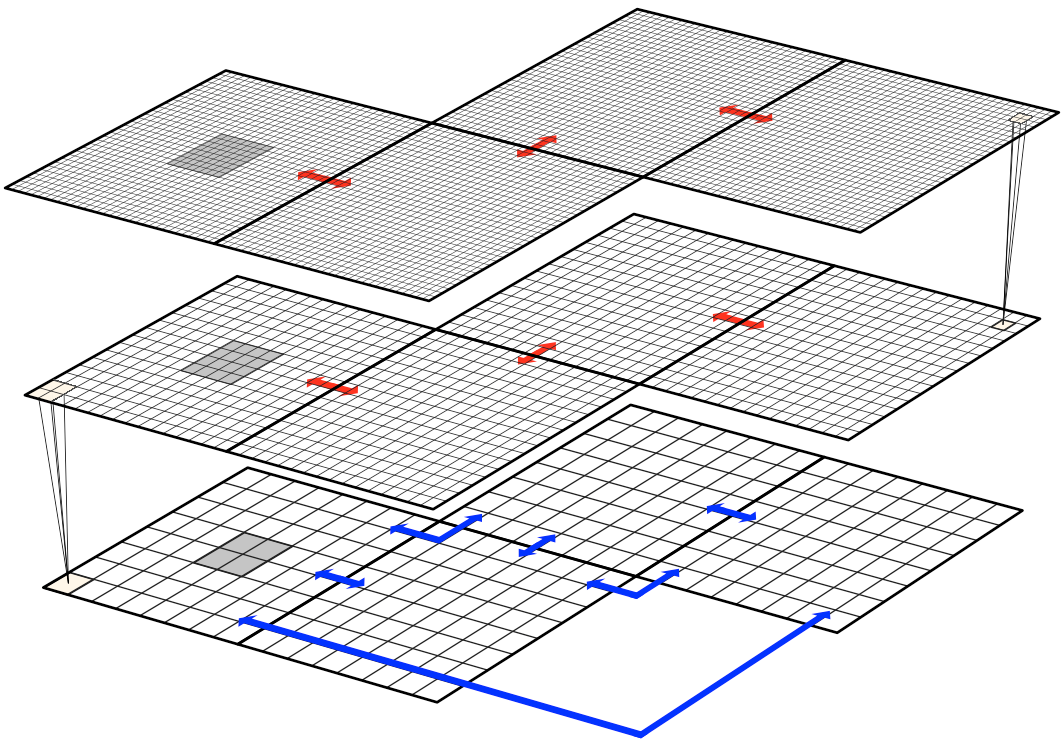
\includegraphics[width=.45\textwidth]{./figures/mg_method.png}};

\foreach \y in {0,1,2} {
   \pgfmathsetlengthmacro{\ypos}{(\y*2.3-3+0.7)*1cm}
   \node at (-7,\ypos) { \small Level \y }; 
}

\draw [->, dashed] (0,-4) -- (0,-5) -- (8,-5) -- (8,5) -- (0,5) -- (0,4);
\node at (4,5.5) { \small Pressure iteration }; 

\def\xposC{-15.5}
\def\yred{2.5}
\def\yblue{1.5}
\node[text=red, anchor=west] (RED) at (\xposC,\yred) { \footnotesize Local communication }; 
\draw [<->, color=red, very thick] ($ (RED.west) - (1,0) $) -- (RED.west);
\node[text=blue, anchor=west] (BLUE) at (\xposC,\yblue) { \footnotesize Global communication }; 
\draw [<->, color=blue, very thick] ($ (BLUE.west) - (1,0) $) -- (BLUE.west);

\def\xposG{-13.5}
\node[inner sep=0pt] (TRANS) at (\xposG,-1.1)
 {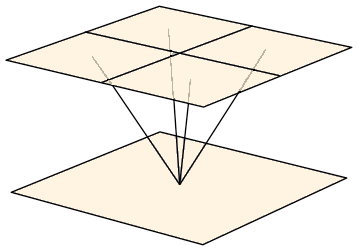
\includegraphics[scale=0.7]{./figures/mg_transfer.png}};
\node at ($(TRANS.south) - (0,0.5)$) { \footnotesize Grid transfer }; 

\end{tikzpicture}
\end{center}
%

\caption{Geometric multigrid method with mesh-wise smoothing for the 2D pipe geometry. Local communication is needed for matrix-vector products, global communication for the solution of the coarse grid problem. }
\label{FIG_SCARC_mg_method}
\end{figure}

For an algorithmic description of this procedure, 
let there be given a hierarchical sequence of $L$ meshes for the domain $\Omega$
with corresponding mesh parameters $0<h^{(L)}< \ldots < h^{(0)}\,,$
where the finest grid is associated with index `$L$' up to index `0' for the coarse grid. On every mesh level 
$l=0, \ldots,L\,,$ the
corresponding Poisson matrix $A^{(l)}$, preconditioning matrix $B^{(l)}$, solution vector $x^{(l)}$ and right hand side vector $b^{(l)}$ are
used.
Further, let ${R^{(l)}}^T$ be a prolongation operator which interpolates a vector from level $l$ to level $l+1$ and
$R^{(l)}$ its corresponding counterpart which restricts a vector vice-versa.

In order to simplify the notation we will subsequently omit the iteration index $k$ used in the basic iteration (\ref{EQ_SCARC_basic_iteration})
and simply use the notation $x_i \leftarrow (\cdot)$
to express that the value on the right hand side is assigned to the left hand side within an iterative process. Thus, the basic iteration on each grid level $l$ now simply reads as
\[ x^{(l)} \leftarrow x^{(l)} + B^{(l)}\, \big(b^{(l)} - A^{(l)} x^{(l)} \big)\,. \]

Based on these definitions the MG-method with smoothing by the preconditioning matrices $B^{(l)}$ reads like summarized below.

\newpage   % remove this depending on layout
\paragraph{\underline{{\bf Multigrid method}\,\,{\boldmath $x^{(l)} \leftarrow MG(l,A^{(l)},b^{(l)},x^{(l)},b^{(l)})$}\,\, for\,\,{\boldmath $l\geq 1$}}} \mbox{} \\[1ex]
Given an initial solution, then compute an approximate solution of $A^{(l)} x^{(l)} =b^{(l)}$ by:
\begin{enumerate}
%
\item {\bf Pre-smoothing:} \\ [1ex]
Perform $k_1$ steps of a basic iteration scheme
\[ x^{(l)} \leftarrow x^{(l)} + B^{(l)}\, \big(b^{(l)} - A^{(l)} x^{(l)} \big)\,. \]
\item {\bf Coarse grid correction:}
%
\begin{enumerate}
\item Restrict the defect to level $l-1$
\[ b^{(l-1)} \leftarrow R^{(l-1)} (b^{(l)} - A^{(l)} x^{(l)} )\,. \]
\item Solve the problem
\[ A^{(l-1)} x^{(l-1)} = b^{(l-1)} \]
in case $\,l=1$ exactly and in case  $l>1$ by $p$-fold recursive application of
\[ x^{(l-1)}  \leftarrow MG(l-1,A^{(l-1)}, b^{(l-1)}, x^{(l-1)}, b^{(l-1)}),\,\]
$p \geq 1\,,$  with $x^{(l-1)}=0$.
\item Correct the solution on level $l$ by the prolonged coarse grid solution
\[ x^{(l)} \leftarrow x^{(l)} + {R^{(l-1)}}^T x^{(l-1)} \,.\]
\end{enumerate}
%
\item {\bf Post-smoothing:} \\[1ex]
Perform $k_2$ steps of a basic iteration scheme
\[ x^{(l)} \leftarrow x^{(l)} + B^{(l)}\, \big(b^{(l)} - A^{(l)} x^{(l)} \big)\,. \]
%
\end{enumerate}

\begin{figure}[htbp]
\begin{center}
\begin{tikzpicture}
[
  scale=0.50,
 every node/.style ={scale=0.5},
]
\node at (-1,0) {\Large Level 0};
\node at (-1,1) {\Large  Level 1};
\node at (-1,2) {\Large  Level 2};
\node at (-1,3) {\Large  Level 3};
\node at (-1,4) {\Large  Level 4};

\draw[-, line width=0.1mm,black!20] (0.8,0)--(28.0,0); 
\draw[-, line width=0.1mm,black!20] (0.8,1)--(28.0,1); 
\draw[-, line width=0.1mm,black!20] (0.8,2)--(28.0,2); 
\draw[-, line width=0.1mm,black!20] (0.8,3)--(28.0,3); 
\draw[-, line width=0.1mm,black!20] (0.8,4)--(28.0,4); 

\node at (29.5,0) {\Large coarse};
\draw[<->, thick, dotted](29.5,0.5)--(29.5,3.5);
\node at (29.5,4) {\Large  fine};

\def \zigzag(#1,#2,#3) {
  \def\coord{{#1}}
  \def\n{#2}
  \def\x{#3}
  \foreach \xi in {0,...,\n} {
      \pgfmathtruncatemacro{\xj}{\xi+1};
      \pgfmathtruncatemacro{\xa}{\xi+\x};
      \pgfmathtruncatemacro{\xb}{\xa+1};
    
      \draw[-,line width=0.6mm](\xa,\coord[\xi])--(\xb,\coord[\xj]); 
  }
}

\zigzag({4,0,4},1,1)
\node at (2,-1) {\bf \LARGE V};

\zigzag({4,0,1,0,2,0,3,0,4},7,4)
\node at (8,-1) {\bf \LARGE F};

\zigzag({4,0,1,0,2,0,1,0,3,0,1,0,2,0,4},13,14)
\node at (22,-1) {\bf \LARGE W};

\end{tikzpicture}

%\includegraphics[height=2.7cm]{\figPath/fig_ver_cycles}
\end{center}
\caption{Different types of multigrid cycles which prescribe the order in which and how often the single levels are run through.}
\label{FIG_SCARC_mg_cycle}
\end{figure}

\newpage  % remove this depending on layout
The number of smoothing steps may depend on the grid level. It is also possible to only apply the pre- or post-smoothing exclusively.
%In the correction step (2c), the prolonged coarse grid solution can also be weighted by an additional relaxation parameter $x^{(l-1)} \leftarrow x^{(l-1)} + \alpha b^{(l)}\, \big(b^{(l)} - A^{(l)} x^{(l-1)} \big)$.
The recursive change between the different grid levels can be performed in several ways, depending on how
often and in which order the the individual levels are passed, see Fig.~\ref {FIG_SCARC_mg_cycle}.


From a computational point of view the V-cycle is the most efficient type because it only needs one single coarse grid solution, but it also behaves the most sensitive to irregularities in the problem.
The most robust, but also the most expensive, is the W cycle. As a good compromise between
the higher computational efficiency of the V-cycle and the larger 
robustness of the W-cycle the F cycle has evolved.
The cost of a complete cycle is only a modest multiple of the cost for a single pass on the finest grid.


All in all, each grid level is responsible for the reduction of a certain range of the error frequencies. The low-frequent components on a finer grid appear as high-frequent components on the next coarser grid. The efficiency of the complete method substantially depends on how good the ranges, which are smoothed on the single grid levels, are adjusted among each other.
%
Besides, there is not only ONE single MG-method but a huge range of variations based on different combinations of its components (smoothers, grid transfer operators and coarse grid solvers) which should best be adapted to the underlying problem.

The upper MG-method can be used for both serial and parallel applications and the same considerations regarding the parallel executability of the single components hold true as for the CG-method before.
%
The solution of the coarse grid problem takes a special position here: It is a very small problem which has to be solved globally such that the relation between computational and communication work is disproportionately bad.
Its global computation implies a logarithmical growth of the communication costs if the number of subdomains is increased. This can be remedied by completely solving the coarse grid problem on a single processor, what in turn is associated with corresponding data transfers and waiting times on the other processors. Nevertheless, by using adequate domain decomposition strategies based on strong smoothers high numerical efficiencies can be achieved, such that usually only a few MG-iterations must be performed and the disadvantages mentioned do not matter that much.


\subsubsection{Summary for the basic iteration} 
All in all it can be stated that both, CG- and MG-methods, are able to reasonably improve the convergence speed of the basic iteration returning the exact solution in a small up to a moderate number of iterations depending on the underlying problem. 

Apart from using the aforementioned globally defined matrix-vector products, these methods incorporate even more globally acting features such as global scalar-products in case of CG or an additional coarse grid problem in case of MG which furthermore contribute to a stronger global coupling. Certainly, the acceleration of convergence speed achieved by these features must be set in relation to the increased computational overhead associated with them.

Due to their already mentioned restriction to different core components, iterative methods prove to be easier and more universally parallelizable than direct ones. In both methods the local solutions are not used as stand-alone solvers but embedded in an outer iteration where they only serve as corrections to the global solution. In this context, the potential of domain decomposition methods can largely be exploited.

